%%%%%%%%%%%%%%%%%%%%%%%%%%%%%%%%%%%%%%%%%%%%%%%%%%%%%%%%%%%%%%%%%%%%%
% In English:
%    This is a Latex template for São Paulo Research Foudation (FAPESP)
%         reports (annual or final).
%    This is the modified version of the original Latex template from
%         following website.
%    Original Source: http://www.howtotex.com
%    For information about FAPESP, check http://www.fapesp.br/en
%    This template targets mainly on reports in Portuguese language.
%    New additions and changes in the latest version:
%        - Added the possibility of including multiple members in the
%          research team, with the commands \memberA{Name of Member A}
%          \memberB{Name of Member B} \memberC{Name of Member C} etc.
%        - Included commands to define project modality and the research
%          agency (if you want to use the same model for other research
%          agencies such as CAPES, CNPq etc).
%
% In Portuguese:
%    Este é um modelo Latex para relatórios (anual ou final) da Fundação
%         de Amparo à pesquisa do Estado de São Paulo (FAPESP).
%    Esta é uma versão modificada do modelo Latex do site supra mencionado.
%    Para informações sobre a FAPESP, verifique http://www.fapesp.br
%    Esse modelo foca principalmente nos relatórios escritos em Português.
%    Novas adições e alterações na última versão:
%       - Foi adicionada a possibilidade de incluir vários membros no
%         grupo de pesquisas, com os comandos \membroA{Nome do Membro A}
%         \membroB{} \membroC{} etc.
%       - Foram incluídos comandos para definir modalidade de projeto e
%         agência de fomento (caso queira utilizar o mesmo modelo para
%         outras agências, CAPES, CNPq etc).
%
% Author/Autor: André Leon Sampaio Gradvohl, Dr.
% Email:        andre.gradvohl@gmail.com
% Lattes CV:    http://lattes.cnpq.br/9343261628675642
% GitHub: http://gradvohl.github.io/
%
% Last update/Última versão: 19/Feb/2018
%
%%%%%%%%%%%%%%%%%%%%%%%%%%%%%%%%%%%%%%%%%%%%%%%%%%%%%%%%%%%%%%%%%%%%%%
\documentclass[12pt]{report}
\usepackage[a4paper]{geometry}
\usepackage[utf8]{inputenc}
\usepackage[english]{babel}
\usepackage[myheadings]{fullpage}
\usepackage[T1]{fontenc}
\usepackage{fancyhdr}
\usepackage{setspace}
\usepackage{sectsty}
\usepackage{url}

%%% iniciar capitulo na mesma pagina (Mateus) %%%
\usepackage{etoolbox}
\makeatletter %inicio da modificacao (iniciar capitulo na msma pag)
\patchcmd{\chapter}{\if@openright\cleardoublepage\else\clearpage\fi}{}{}{}
\makeatother %fim da modificacao
%%% iniciar capitulo na mesma pagina (Mateus) %%%

%%------
%% Comandos gerais
%% Observação: o arquivo "comandos.tex" tem que estar presente.
%%------
%%%%%%%%%%%%%%%%%%%%%%%%%%%%%%%%%%%%%%%%%%%%%%%%%%%%%%%%%%%%%%%%%%%%%
% In English:
%    This is a list of commands specification for FAPESP reports.
%
% In Portuguese:
%    Esta é uma lista de especificação de comandos para relatórios
% da Fundação de Amparo à pesquisa do Estado de São Paulo (FAPESP).
%
% Author/Autor: André Leon Sampaio Gradvohl, Dr.
% Email:        andre.gradvohl@gmail.com
% Lattes CV:    http://lattes.cnpq.br/9343261628675642
%
% Last update/Última versão: 11/Sep/2016
%%%%%%%%%%%%%%%%%%%%%%%%%%%%%%%%%%%%%%%%%%%%%%%%%%%%%%%%%%%%%%%%%%%%%%

\newcommand{\HRule}[1]{\rule{\linewidth}{#1}}
\setcounter{tocdepth}{3}
\setcounter{secnumdepth}{3}

\newcommand{\titulo}[1]{\def\meuTitulo{#1}}
\newcommand{\tituloIngles}[1]{\def\meuTituloIngles{#1}}
\newcommand{\numProjeto}[1]{\def\numFAP{#1}}
\newcommand{\tipoRelatorio}[1]{\def\tipoRelat{#1 }} %o espaço depois do #1 é importante
\newcommand{\modalidadeProjeto}[1]{\def\modProjeto{#1}}
\newcommand{\agFomento}[2]{\def\agFom{#1} \def\siglaAgFom{#2}} %extenso Sigla
\newcommand{\autor}[1]{\def\nomeAutor{#1}}
\newcommand{\cidade}[1]{\def\nomeCidade{#1}}
\newcommand{\universidade}[1]{\def\nomeUniversidade{#1}}
\newcommand{\faculdade}[1]{\def\nomeFaculdade{#1}}
\newcommand{\periodoVigencia}[1]{\def\periodVig{#1}}
\newcommand{\periodoRelatorio}[1]{\def\periodRelat{#1}}
\newcommand{\orientador}[1]{\def\nomeOrientador{#1}}

\newcommand\namegroup[3]{%
   \begin{minipage}[t]{0.4\textwidth}
   \hspace{0.6cm}
   \begin{tikzpicture}
   \node[anchor=south east,inner sep = 0](signF){\includegraphics[width=#3]{#2}};
   \end{tikzpicture}
   \vspace*{0.1cm}  % leave some space above the horizontal line
   \hrule
   \vspace{1mm} % just a bit more whitespace below the line
   \centering
   \begin{tabular}[t]{c}
   #1
   \end{tabular}
   \end{minipage}}

\author{}
\date{}

%Definição de membros da equipe de pesquisas
\newcommand{\membroA}[1]{\def\nomeMembroA{#1}}
\newcommand{\membroB}[1]{\def\nomeMembroB{#1}}
\newcommand{\membroC}[1]{\def\nomeMembroC{#1}}
\newcommand{\membroD}[1]{\def\nomeMembroD{#1}}
\newcommand{\membroE}[1]{\def\nomeMembroE{#1}}
\newcommand{\membroF}[1]{\def\nomeMembroF{#1}}

\newcommand{\Figure}[1]{Figura~\ref{fig:#1}}
\newcommand{\Table}[1] {Tabela~\ref{#1}}
\newcommand{\Equation}[1] {Equa\c{c}\~ao~\ref{#1}}
\newcommand{\addFigure}[3] { %Parametros scale, fig_name, caption
    \begin{figure}[!hbt]
      \centering
      \includegraphics[scale=#1]{figures/}
      \caption{#3}\label{fig:#2}
    \end{figure}
}

\newcommand{\geraTitulo}{
\clearpage
\begin{titlepage}
  \begin{center}
      \vspace*{-3cm}
       { \setstretch{.5}
         \textsc{\nomeUniversidade} \\
         \HRule{.2pt}\\
         \textsc{\nomeFaculdade}
       }

       \vspace{5.5cm}

       \Large \textbf{\textsc{\meuTitulo}}
 	  \HRule{1.5pt} \\ [0.5cm]
       \linespread{1}
       \large Final report on the activities
       %\ifdefined\tipoRelat
       %     \tipoRelat
       %\fi
       of the
       \ifdefined\modProjeto
           \modProjeto
       \fi
       ~project supported by the \agFom. \\
   	   \HRule{1.5pt} \\ [0.5cm]

       \ifdefined\numFAP
          Grant \texttt{\#\numFAP}, \siglaAgFom
          \\ [0.5cm]
       \fi
        Author: \nomeAutor \\
        Advisor: \nomeOrientador \\[5.cm]

        % aqui começa a adicao das linhas de assinatura
        %Aluno: \tikz\draw [thick,solid] (0,0) -- (6,0); \\[.5cm]
        %Orientador: \tikz\draw [thick,solid] (0,0) -- (5.5,0);


        %% Assinatura assinatura ASSINATURA
        %\namegroup{Researcher}{example-image-a}
        \namegroup{Researcher}{fig/assinatura-mateus.png}{5cm}
        \hspace{1.5cm}
        \namegroup{Advisor}{fig/placeholder.png}{1cm}

        %\begin{minipage}[t]{0.4\textwidth}
        %\vspace*{1.5cm}
        %\hrule
        %\vspace{1mm}
        %\centering
        %\begin{tabular}[t]{c}
        %Aluno
        %\end{tabular}
        %\hspace{1.5cm}
        %\begin{minipage}[t]{0.4\textwidth}
        %\vspace*{1.5cm}
        %\hrule
        %\vspace{1mm}
        %\centering
        %\begin{tabular}[t]{c}
        %Aluno
        %\end{tabular}
        %\end{minipage}
        %%\hfill

        \vfill

        {\normalsize  \nomeCidade, \today}
 \end{center}
 \end{titlepage}
}

\usepackage{titlesec}
\titleformat{\chapter}{\normalfont\LARGE\bfseries}{\thechapter}{1em}{}
\titlespacing*{\chapter}{0pt}{3.5ex plus 1ex minus .2ex}{2.3ex plus .2ex}

%----------------------------------------------------------------------
% Cabeçalho e rodapé
%----------------------------------------------------------------------
\pagestyle{fancy}
\fancyhf{} % Limpa todos os campos de header and footer fields
\renewcommand{\headrulewidth}{0pt}
\fancyfoot[R]{\thepage}

\addto\captions{\renewcommand{\contentsname}{Summary}}
\addto\captions{\renewcommand{\bibname}{Bibliography}}

%------
% Resumo e Abstract
%------
%%\newcommand{\Resumo}[1]{
%%   \begin{otherlanguage}{portuguese}
%%       \addcontentsline{toc}{chapter}{Resumo}
%%       \begin{abstract} \thispagestyle{plain} \setcounter{page}{2}
%%          #1
%%        \end{abstract}
%%   \end{otherlanguage}
%%} %end \Resumo

\newcommand{\Abstract}[1]{
   \begin{otherlanguage}{english}
      \addcontentsline{toc}{chapter}{Abstract}
      \begin{abstract} \thispagestyle{plain} \setcounter{page}{3}
       #1
      \end{abstract}
    \end{otherlanguage}
} %end \abstract

%------
% Folha de rosto
%------


\newcommand{\folhaDeRosto}{
   \chapter*{Project}
   \addcontentsline{toc}{chapter}{General Project Information}
   \begin{itemize}
      \item Title:
            \begin{itemize}\item[] \textbf{\meuTitulo} \end{itemize}
      \item Advisor:
            \begin{itemize}\item[]\textbf{Prof. \nomeOrientador}\end{itemize}
      \item Project host institution:
            \begin{itemize}
               \item[]\textbf{\nomeFaculdade \ da \nomeUniversidade}
            \end{itemize}
      \item Research team:
            \begin{itemize}
               \ifdefined\nomeMembroA
                 \item[]\textbf{\nomeMembroA}
               \else
                 \item[]\textbf{\nomeAutor}
               \fi
               \ifx\nomeMembroB\undefined\else \item[]\textbf{\nomeMembroB}\fi
               \ifx\nomeMembroC\undefined\else \item[]\textbf{\nomeMembroC}\fi
               \ifx\nomeMembroD\undefined\else \item[]\textbf{\nomeMembroD}\fi
               \ifx\nomeMembroE\undefined\else \item[]\textbf{\nomeMembroE}\fi
               \ifx\nomeMembroF\undefined\else \item[]\textbf{\nomeMembroF}\fi
             \end{itemize}

          \ifdefined \numFAP
             \item Research project number:
             \begin{itemize}
                 \item[]\textbf{\numFAP}
             \end{itemize}
          \fi
       \item Validity period:
            \begin{itemize}
               \item[]\textbf{\periodVig}
            \end{itemize}
       \item Period covered by this scientific report:
            \begin{itemize}
               \item[]\textbf{\periodRelat}
            \end{itemize}
   \end{itemize}
   \clearpage
}


%\newcommand{\folhaDeRosto}{
%   \chapter*{Informações Gerais do Projeto}
%   \addcontentsline{toc}{chapter}{Informações Gerais do Projeto}
%   \begin{itemize}
%      \item Título do projeto:
%            \begin{itemize}\item[] \textbf{\meuTitulo} \end{itemize}
%      \item Nome do pesquisador responsável:
%            \begin{itemize}\item[]\textbf{Prof. \nomeOrientador}\end{itemize}
%      \item Instituição sede do projeto:
%            \begin{itemize}
%               \item[]\textbf{\nomeFaculdade \ da \nomeUniversidade}
%            \end{itemize}
%      \item Equipe de pesquisa:
%            \begin{itemize}
%               \ifdefined\nomeMembroA
%                 \item[]\textbf{\nomeMembroA}
%               \else
%                 \item[]\textbf{\nomeAutor}
%               \fi
%               \ifx\nomeMembroB\undefined\else \item[]\textbf{\nomeMembroB}\fi
%               \ifx\nomeMembroC\undefined\else \item[]\textbf{\nomeMembroC}\fi
%               \ifx\nomeMembroD\undefined\else \item[]\textbf{\nomeMembroD}\fi
%               \ifx\nomeMembroE\undefined\else \item[]\textbf{\nomeMembroE}\fi
%               \ifx\nomeMembroF\undefined\else \item[]\textbf{\nomeMembroF}\fi
%             \end{itemize}
%
%          \ifdefined \numFAP
%             \item Número do projeto de pesquisa:
%             \begin{itemize}
%                 \item[]\textbf{\numFAP}
%             \end{itemize}
%          \fi
%       \item Período de vigência:
%            \begin{itemize}
%               \item[]\textbf{\periodVig}
%            \end{itemize}
%       \item Período coberto por este relatório científico:
%            \begin{itemize}
%               \item[]\textbf{\periodRelat}
%            \end{itemize}
%   \end{itemize}
%   \clearpage
%}

\usepackage[brazilian]{babel}
\usepackage[left=2.5cm,right=2.5cm,top=3cm,bottom=2.5cm]{geometry}
\usepackage{mathtools}
\usepackage{amsthm}
\usepackage{amsmath}
%\usepackage{nccmath}
\usepackage{amssymb}
\usepackage{amsfonts}
\usepackage{physics}
%\usepackage{dsfont}
%\usepackage{mathrsfs}

\usepackage{titling}
\usepackage{indentfirst}

\usepackage{bm}
\usepackage[dvipsnames]{xcolor}
\usepackage{cancel}

\usepackage{xurl}
\usepackage[colorlinks=true]{hyperref}

\usepackage{float}
\usepackage{graphicx}
%\usepackage{tikz}
\usepackage{caption}
\usepackage{subcaption}

%%%%%%%%%%%%%%%%%%%%%%%%%%%%%%%%%%%%%%%%%%%%%%%%%%%

\newcommand{\eps}{\epsilon}
\newcommand{\vphi}{\varphi}
\newcommand{\cte}{\text{cte}}

\newcommand{\N}{\mathbb{N}}
\newcommand{\Z}{\mathbb{Z}}
\newcommand{\Q}{\mathbb{Q}}
\newcommand{\R}{\vb{R}}
\newcommand{\C}{\mathbb{C}}
\renewcommand{\S}{\hat{S}}
%\renewcommand{\H}{\s{H}}

\renewcommand{\a}{\vb{a}}
\newcommand{\nn}{\hat{n}}
\renewcommand{\d}{\dagger}
\newcommand{\up}{\uparrow}
\newcommand{\down}{\downarrow}

\newcommand{\0}{\vb{0}}
%\newcommand{\1}{\mathds{1}}
\newcommand{\E}{\vb{E}}
\newcommand{\B}{\vb{B}}
\renewcommand{\v}{\vb{v}}
\renewcommand{\r}{\vb{r}}
\renewcommand{\k}{\vb{k}}
\newcommand{\p}{\vb{p}}
\newcommand{\q}{\vb{q}}
\newcommand{\F}{\vb{F}}

\newcommand{\s}{\sigma}
%\newcommand{\prodint}[2]{\left\langle #1 , #2 \right\rangle}
\newcommand{\cc}[1]{\overline{#1}}
\newcommand{\Eval}[3]{\eval{\left( #1 \right)}_{#2}^{#3}}

\newcommand{\unit}[1]{\; \mathrm{#1}}

\newcommand{\n}{\medskip}
\newcommand{\e}{\quad \mathrm{e} \quad}
\newcommand{\ou}{\quad \mathrm{ou} \quad}
\newcommand{\virg}{\, , \;}
\newcommand{\ptodo}{\forall \,}
\renewcommand{\implies}{\; \Rightarrow \;}
%\newcommand{\eqname}[1]{\tag*{#1}} % Tag equation with name

\setlength{\droptitle}{-7em}

\theoremstyle{plain}
\newtheorem{theorem}{Teorema}[section]
%\newtheorem{defi}[theorem]{Definição}
\newtheorem{lemma}[theorem]{Lema}
%\newtheorem{corol}[theorem]{Corolário}
%\newtheorem{prop}[theorem]{Proposição}
%\newtheorem{example}{Exemplo}
%
%\newtheorem{inneraxiom}{Axioma}
%\newenvironment{axioma}[1]
%  {\renewcommand\theinneraxiom{#1}\inneraxiom}
%  {\endinneraxiom}
%
%\newtheorem{innerpostulado}{Postulado}
%\newenvironment{postulado}[1]
%  {\renewcommand\theinnerpostulado{#1}\innerpostulado}
%  {\endinnerpostulado}
%
%\newtheorem{innerexercise}{Exercício}
%\newenvironment{exercise}[1]
%  {\renewcommand\theinnerexercise{#1}\innerexercise}
%  {\endinnerexercise}
%
%\newtheorem{innerthm}{Teorema}
%\newenvironment{teorema}[1]
%  {\renewcommand\theinnerthm{#1}\innerthm}
%  {\endinnerthm}
%
\newtheorem{innerlema}{Lema}
\newenvironment{lema}[1]
  {\renewcommand\theinnerlema{#1}\innerlema}
  {\endinnerlema}
%
%\theoremstyle{remark}
%\newtheorem*{hint}{Dica}
%\newtheorem*{notation}{Notação}
%\newtheorem*{obs}{Observação}

%
%%-----
%% Página de título
%% Observação: As definições que aparecem a seguir comporão a
%%             página de título e a folha de rosto.
%%-----
%% Define o nome da universidade onde o projeto foi desenvolvido.
\universidade{Universidade de São Paulo (USP)}
%
%% Define o nome da faculdade onde o projeto foi desenvolvido.
\faculdade{Instituto de Física}
%
%% Define o título do projeto.
\titulo{Multi-orbital topological Anderson models for twisted bilayer graphene}
%
%% Define a agencia de Fomento e a abreviatura. O primeiro argumento é o
%% nome por extenso e o segundo a abreviatura.
%% Ambos os argumentos são obrigatórios
\agFomento{São Paulo Research Foundation}{FAPESP}
%
%% Define o tipo de relatório. Pode ser Anual ou Final.
%% Não é obrigatório definir o tipo de relatório.
%\tipoRelatorio{Final}
%
%% Define a modalidade de Projeto. Pode ser temático, regular, etc.
\modalidadeProjeto{Master's degree}
%
%% Define o número do projeto.
%% Não é obrigatório definir o número do projeto.
\numProjeto{2023/02913-5}
%
%% Define o autor do relatório.
\autor{Mateus Marques}
\orientador{Dr. Luis Gregório G. V. Dias da Silva}
%
%% Define a equipe do projeto (incluindo o pesquisador responsável no comando \membroA{}
\membroA{Mateus Marques}
%% Inclua os demais membros do grupo (máximo +5)
\membroB{Luis Gregório G. V. Dias da Silva}
%\membroC{Francisco}
%\membroD{Joao}
%\membroE{Antonio}
%\membroF{José}
%
%% Define o período da vigência do Projeto.
\periodoVigencia{January 1, 2023 to December 31, 2024}
%
%% Define o período coberto pelo relatório.
\periodoRelatorio{July 16, 2024 to \today}  % o período de entrega passado encerrou em 15 de julho. por isso 16 de julho
%
%% Define a cidade onde o projeto foi desenvolvido.
\cidade{São Paulo}

\newcommand{\ALERT}[1]{\textcolor{red}{#1}}

%%-----
%% Página de título
%% Observação: Os comandos a seguir não devem ser mudados,
%%             exceto caso necessário.
%%-----
\begin{document}
%
%% Define a numeração em romanos.
\pagenumbering{roman}
%
%% Gera a folha de título.
\geraTitulo
%
%% Gera a folha de rosto.
\folhaDeRosto
%
%% Escreva aqui o resumo em português. Fica no Resumo do Projeto Proposto
%\Resumo{
%Neste projeto estamos interessado apenas no valor da bolsa. Não fizemos praticamente
%nada nesse tempo e não pretendemos fazer. Eu apenas pretendo entregar este relatório
%para ficar tudo certo.
%}
%
%% Escreva aqui o resumo em inglês. NAO PRECISA
%\Abstract{
%Same thing but in english.
%}
%
%% Adicionará o sumário.
%% Mantenha o \thispagestyle{empty} e \clearpage
\tableofcontents
\thispagestyle{empty}
\clearpage
%
%% Define a numeração em arábicos.
\pagenumbering{arabic}

%%-----
%% Formatação do título da seção
%%-----
\sectionfont{\scshape}

%%-----
%% Corpo do texto
%%-----


%%-----
%% Resumo do projeto
%%-----
\chapter{Summary of the Research Project} \label{chp:abstract}

Twisted Bilayer Graphene (TBG) is a fascinating system that displays a plethora of intriguing physical phenomena such as correlated insulators \cite{cao2018_correlated}, superconductivity \cite{cao2018}, and unconventional quantum Hall effects \cite{unconv_QHE_tbg_2006}, among others. Several recent experiments have demonstrated the rich electronic properties of TBG, which exhibits correlated insulating and superconducting phases. Despite the vast amount of experimental data, there remain several open questions regarding the theoretical description of this material in different regimes. While there is some consensus that these phenomena are related to the formation of flat bands near the Fermi level, captured by non-interacting band structure models \cite{macdonald2011}, describing TBG as a strongly correlated system remains challenging.

This Master's project focuses on the Magic-Angle Twisted Bilayer Graphene (MATBG) system, aiming to employ symmetry and topological analyses to describe it through a Topological Heavy Fermion (THF) model \cite{topoheavyfermion2022}. The study combines analytical and numerical approaches to explore the low-energy physics of the THF model, emphasizing emergent energy scales and symmetries. The project addresses two primary objectives:
\begin{enumerate}[label=(\alph*)]
\item understanding the symmetry and topological characteristics of TBG, and
\item developing a mapping of the Bistritzer-MacDonald model to a THF model in the low-energy regime.
\end{enumerate}

For objective (a), Sections \ref{sec:grouptheory} and \ref{sec:topological_quantum_chemistry} details our progress in understanding group and representation theory and their application to Topological Quantum Chemistry (TQC) \cite{topological_quantum_chemistry2017}. TQC provides a framework to identify topological properties of band structures based on symmetry and real-space considerations. A crucial concept here is the Wannier obstruction \cite{zou2018}, which arises from the non-trivial topology of the bands. This obstruction reflects the inability to construct exponentially localized Wannier functions that preserve all symmetries of the band structure.

Objective (b) addresses resolving the Wannier obstruction identified in (a). The THF model provides a fully symmetric approach, reformulating and mapping the interacting MATBG system as a topological heavy fermion system \cite{topoheavyfermion2022}. This involves using the Bilbao Crystallographic Server \cite{bilbao_1, bilbao_2} to compute the Elementary Band Representations (EBRs) for the space group \( P6'2'2 \) (\#177.151 in the International Table) of the Bistritzer-MacDonald model. By comparing these EBRs with the model's representations at high-symmetry points, we aim to develop a mapping that preserves all symmetries, establishes a Wannier basis, and facilitates the formulation of an interacting model analogous to heavy fermions coupled with nearly free electrons.

\pagebreak


\chapter{Accomplishments in the period} \label{chp:accomplishments}

Throughout the period covered in this report, our work advanced in three main areas: deepening our understanding of advanced Group and Representation Theory concepts, establishing a foundation in Topological Quantum Chemistry, and applying these frameworks to analyze the Topological Heavy Fermion (THF) model. The key developments are summarized as follows:

\begin{itemize}
\item \textit{Group and Representation Theory}:
We studied references \cite{dresselhaus, evarestov, barata_representacoes, magnetic_structures2012, michael_glazer2012_space_groups, thesis_rennella} to enhance our knowledge of group theory. This included the process of \textit{induction of representations}, which is crucial for mathematically defining topological bands, and the concept of \textit{magnetic space groups} -- space groups incorporating the time-reversal symmetry. These studies are particularly relevant since the Bistritzer-Macdonald (BM) model is associated with the magnetic space group \( P6'2'2 \).

\item \textit{Topological Quantum Chemistry (TQC)}:
We explored the fundamentals of TQC as outlined in \cite{topological_quantum_chemistry2017, building_blocks2018, lectures_tms2017}, focusing on understanding Wannier obstruction. This involves applying coset decompositions of the full space group into site-symmetry groups corresponding to Wyckoff positions. Starting with a representation \( \rho \) of the site-symmetry group \( G_\q \), we construct an induced representation \( \rho_G = \rho \uparrow G \), known as a \textit{band representation}. TQC allows the classification of materials by determining if their bands are direct sums of elementary band representations (EBRs). If not, the system is identified as topological.

\item \textit{Topological Heavy Fermion (THF) model}:
We applied the TQC framework to analyze the MATBG system. For the BM model, the high-symmetry point representations of the bands are \( \Gamma_1 \oplus \Gamma_2 \), \( M_1 \oplus M_2 \), and \( K_2 K_3 \) \cite{all_magic_angles, bernevig_II_2021} at points \( \Gamma \), \( M \), and \( K \), respectively. Comparing these with the EBR tables for the space group \( P6'2'2 \) confirms that the system is topological and exhibits a Wannier obstruction. To address this issue, we studied the THF model \cite{topoheavyfermion2022}, which maps the low-energy bands of MATBG into a heavy fermion problem. This model resolves the Wannier obstruction by coupling \( f \)-electrons (flat bands, heavy) with \( c \)-electrons (nearly free), providing a complete description that includes all emergent symmetries.
\end{itemize}

%%%%%%%%%%%%%%%%%%%%%%%%%%%%%%%%%%%%%%%%%%%%%%%%%%%%%%%%%%%%%%%%%%%%%%%%%%%%%%%%%%%%%%%%%%%%%%%%%%
\section{Group and Representation Theory} \label{sec:grouptheory}
%%%%%%%%%%%%%%%%%%%%%%%%%%%%%%%%%%%%%%%%%%%%%%%%%%%%%%%%%%%%%%%%%%%%%%%%%%%%%%%%%%%%%%%%%%%%%%%%%%

%%%%%%%%%%%%%%%%%%%%%%%%%%%%%%%%%%%%%%%%%%%%%%%%%%%%%%%%%%%%%%%%%%%%%%%%%%%%%%%%%%%%%%%%%%%%%%%%%%
\subsection{Induction and Subduction of Representations} \label{subsec:induction_subduction}
%%%%%%%%%%%%%%%%%%%%%%%%%%%%%%%%%%%%%%%%%%%%%%%%%%%%%%%%%%%%%%%%%%%%%%%%%%%%%%%%%%%%%%%%%%%%%%%%%%

\begin{definition}[\textbf{Subduction}] \label{def:subduction_defi}
Let $H \subseteq G$ be a subgroup and $\Pi: G \to \GL(V)$ a representation of $G$. We can naturally construct of a representation $\rho: H \to \GL(V)$ of $H$ on $V$ by restricting $\Pi$ to elements of $H$:
\begin{equation} \label{eq:subduction_defi}
\rho(h) = \Pi(h), \quad \forall \, h \in H \subseteq G.
\end{equation}
We denote $\rho = \Pi \downarrow H$ and is called the \textit{subduction} of $\Pi$ to the subgroup $H$.
\end{definition}


%\begin{example} \label{ex:C3_D3_subduction_example}
%$H = \{E, \Ct, \Ctn{2}\} \subseteq G = D_3$ and $\Pi = \Gamma_2$ as defined in Example \ref{ex:2x2_rep}. The subduced representation $\rho = \Pi \downarrow H$ is obtained by using the matrices $\Pi(h)$, for $h = E, \Ct, \Ctn{2}$.
%\begin{equation} \label{eq:rho_subduced_C3_D3_subduction_example}
%\rho(E) =
%\begin{pmatrix}
%1 & 0 \\
%0 & 1
%\end{pmatrix},
%\quad
%\rho(\Ct) =
%\begin{pmatrix}
%\cos(\frac{2\pi}{3}) & \sin(\frac{2\pi}{3}) \\
%-\sin(\frac{2\pi}{3}) & \cos(\frac{2\pi}{3})
%\end{pmatrix},
%\quad
%\rho(\Ctn{2}) =
%\begin{pmatrix}
%\cos(\frac{4\pi}{3}) & \sin(\frac{4\pi}{3}) \\
%-\sin(\frac{4\pi}{3}) & \cos(\frac{4\pi}{3})
%\end{pmatrix}.
%\end{equation}
%
%The original representation \(\Pi\) includes additional matrices not present in \(\rho\):
%\begin{equation} \label{eq:Pi_C3_D3_subduction_example}
%\Pi(\sv) =
%\begin{pmatrix}
%1 & 0 \\
%0 & 1
%\end{pmatrix},
%\;
%\Pi(\svp) = \Pi(\sv \Ct) =
%\begin{pmatrix}
%-\frac{1}{2} & \frac{\sqrt{3}}{2} \\
%\frac{\sqrt{3}}{2} & \frac{1}{2}
%\end{pmatrix},
%\;
%\Pi(\svpp) = \Pi(\sv \Ctn{2}) =
%\begin{pmatrix}
%-\frac{1}{2} & -\frac{\sqrt{3}}{2} \\
%-\frac{\sqrt{3}}{2} & \frac{1}{2}
%\end{pmatrix},
%\end{equation}
%As discussed in Example \ref{ex:irrep_Gamma12_example}, \(\Pi = \Gamma_2\) is irreducible because its six matrices cannot be transformed into block diagonal form through any conjugate transformation \(A \Pi(g) A^{-1}\), \(\forall g \in D_3\).
%
%However, if we consider only the three matrices in Equation \ref{eq:rho_subduced_C3_D3_subduction_example}, they can be transformed into block diagonal form through the following conjugation by \(A\):
%\begin{equation} \label{eq:subduction_can_be_reducible_example}
%\rho(E) =
%A
%\begin{pmatrix}
%1 & 0 \\
%0 & 1
%\end{pmatrix}
%A^{-1},
%\quad
%\rho(\Ct) =
%A
%\begin{pmatrix}
%e^{-\frac{2\pi i}{3}} & 0 \\
%0 & e^{\frac{2\pi i}{3}}
%\end{pmatrix}
%A^{-1},
%\quad
%\rho(\Ctn{2}) =
%A
%\begin{pmatrix}
%e^{-\frac{4\pi i}{3}} & 0 \\
%0 & e^{\frac{4\pi i}{3}}
%\end{pmatrix}
%A^{-1},
%\quad
%\end{equation}
%\begin{equation} \label{eq:A_matrix_that_diagonalizes}
%A =
%\begin{pmatrix}
%i & -i \\
%1 & 1
%\end{pmatrix}.
%\end{equation}
%Therefore, we can assert that \(\rho\) is a direct sum of two one-dimensional representations, \(\{1, e^{-\frac{2\pi i}{3}}, e^{-\frac{4\pi i}{3}}\}\) and \(\{1, e^{\frac{2\pi i}{3}}, e^{\frac{4\pi i}{3}}\}\), making it reducible. This demonstrates that the subduction of an irreducible representation can result in a reducible one.
%\end{example}



\begin{definition}[\textbf{Induction}] \label{def:induction_defi}
Let $H$ be a subgroup of a finite group $G$ and $\Pi: H \to \GL(V)$ be a representation of $H$ on a $n$-dimensional vector space $V$. Let $R = \{g_1, \ldots, g_m\} \subseteq G$ be a full set of representatives of the left cosets in $G/H$, where $m = \abs{G/H}$. Consider the following $(m\cdot n)$-dimensional vector space
\begin{equation} \label{eq:W_vectorspace_induction_copies}
W = \bigoplus_{i=1}^m g_i V = \qty{w = \bigoplus_{i=1}^n (g_i, v_i) \;\bigg|\; v_i \in V_i},
\end{equation}
where each $g_i V$ is an isomorphic labelled copy of $V$, defined by
\begin{equation} \label{eq:giV_vectorspace_labelled_copy}
g_i V = \{ (g_i, v) \mid g_i \in G, v \in V\}, \quad
\alpha (g_i, u) + \beta (g_i, v) = (g_i, \alpha u + \beta v).
\end{equation}

For each $g \in G$ and $g_i \in R$ there is an $h_i \in H$ and a permutation index $j(i) \in \{1, \ldots, m\}$ such that $g g_i = g_{j(i)} h_i$. The \textit{induced} representation $\rho: G \to \GL(W)$, denoted by $\rho = \Pi \uparrow G$, is defined by the action on an element $w = \bigoplus_{i=1}^{m} (g_i, v_i) \in W$:
\begin{equation} \label{eq:induced_rep_action_defi}
\rho(g) w = \bigoplus_{i=1}^{m} \qty(g_{j(i)}, \Pi(h_i) v_i) \in W.
\end{equation}
\end{definition}


%\begin{example} \label{ex:induced_rep_D3D6}
%Take $G = D_6$, $H = D_3$ and $\Pi = \Gamma_2: H \to \GL(\mathbb{R}^2)$ from Example \ref{ex:2x2_rep}. Using the coset decomposition of $D_6$ from Example \ref{ex:coset_decomp_D3D6}, we obtain the set of coset representatives $R = \{g_1=E, g_2=\sd\}$. Let us calculate the actions of $\rho = \Pi \uparrow G$ for the generators $\{\Cs, \sd, \sv\}$.
%
%\n
%
%$g = \Cs$:
%
%$g_1 = E \implies g g_1 = \Cs E = \Cs = \sd \svpp = g_2 h_1$, where $j(1) = 2$ and $h_1 = \svpp$.
%
%$g_2 = \sd \implies g g_2 = \Cs \sd = \svp = E \svp = g_1 h_2$, where $j(2) = 1$ and $h_2 = \svp$.
%
%\begin{equation} \label{eq:Pi_h1_Pi_h2_example_inducedrep_D6}
%\Pi(h_1) = \Pi(\sv) \Pi(\Ctn{2}) =
%\begin{pmatrix}
%-\frac{1}{2} & -\frac{\sqrt{3}}{2} \\
%-\frac{\sqrt{3}}{2} & \frac{1}{2}
%\end{pmatrix},
%\quad
%\Pi(h_2) = \Pi(\sv) \Pi(\Ct) =
%\begin{pmatrix}
%-\frac{1}{2} & \frac{\sqrt{3}}{2} \\
%\frac{\sqrt{3}}{2} & \frac{1}{2}
%\end{pmatrix}.
%\end{equation}
%
%On the basis $(w_{11}, w_{12}, w_{21}, w_{22})$, where $w_{ij} = (g_i, e_j)$ and $(e_1, e_2)$ is a basis of $\mathbb{R}^2$, we have
%\begin{equation} \label{eq:rhoC6_w11_example_inducedrep_D6}
%\rho(\Cs) w_{11} = (g_{j(1)}, \Pi(h_1) e_1) = \qty(g_2, -\frac{1}{2}e_1 - \frac{\sqrt{3}}{2}e_2)
%= -\frac{1}{2} w_{21} - \frac{\sqrt{3}}{2} w_{22},
%\end{equation}
%
%\begin{equation} \label{eq:rhoC6_w12_example_inducedrep_D6}
%\rho(\Cs) w_{12} = (g_{j(1)}, \Pi(h_1) e_2) = \qty(g_2, -\frac{\sqrt{3}}{2}e_1 + \frac{1}{2}e_2)
%= -\frac{\sqrt{3}}{2} w_{21} + \frac{1}{2} w_{22},
%\end{equation}
%
%\begin{equation} \label{eq:rhoC6_w21_example_inducedrep_D6}
%\rho(\Cs) w_{21} = (g_{j(2)}, \Pi(h_2) e_1) = \qty(g_1, -\frac{1}{2}e_1 + \frac{\sqrt{3}}{2}e_2)
%= -\frac{1}{2} w_{11} + \frac{\sqrt{3}}{2}w_{12},
%\end{equation}
%
%\begin{equation} \label{eq:rhoC6_w22_example_inducedrep_D6}
%\rho(\Cs) w_{22} = (g_{j(2)}, \Pi(h_2) e_2) = \qty(g_1, \frac{\sqrt{3}}{2}e_1 + \frac{1}{2}e_2)
%= \frac{\sqrt{3}}{2} w_{11} + \frac{1}{2}w_{12},
%\end{equation}
%
%\begin{equation} \label{eq:rhoC6_matrix_example_inducedrep_D6}
%\rho(\Cs) =
%\begin{pmatrix}
%\rho_{1111} & \rho_{1112} & \rho_{1211} & \rho_{1212} \\
%\rho_{1121} & \rho_{1122} & \rho_{1221} & \rho_{1222} \\
%\rho_{2111} & \rho_{2112} & \rho_{2211} & \rho_{2212} \\
%\rho_{2121} & \rho_{2122} & \rho_{2221} & \rho_{2222} \\
%\end{pmatrix}
%=
%\begin{pmatrix}
%0                   & 0                   & -\frac{1}{2}       & \frac{\sqrt{3}}{2} \\
%0                   & 0                   & \frac{\sqrt{3}}{2} & \frac{1}{2}        \\
%-\frac{1}{2}        & -\frac{\sqrt{3}}{2} & 0                  & 0                  \\
%-\frac{\sqrt{3}}{2} & \frac{1}{2}         & 0                  & 0                  \\
%\end{pmatrix}
%=
%\begin{pmatrix}
%0 & \Pi(h_2) \\
%\Pi(h_1) & 0
%\end{pmatrix}.
%\end{equation}
%
%\n
%
%$g = \sd$:
%
%$g_1 = E \implies g g_1 = \sd E = g_2 h_1$, where $j(1) = 2$ and $h_1 = E$.
%
%$g_2 = \sd \implies g g_2 = E = E E = g_1 h_2$, where $j(2) = 1$ and $h_2 = E$.
%\begin{equation} \label{eq:rhosd_matrix_example_inducedrep_D6}
%\rho(\sd) =
%\begin{pmatrix}
%0 & \Pi(h_2) \\
%\Pi(h_1) & 0
%\end{pmatrix}
%=
%\begin{pmatrix}
%0 & 0 & 1 & 0 \\
%0 & 0 & 0 & 1 \\
%1 & 0 & 0 & 0 \\
%0 & 1 & 0 & 0 \\
%\end{pmatrix}.
%\end{equation}
%
%\n
%
%$g = \sv$:
%
%$g_1 = E \implies g g_1 = E \sv = g_1 h_1$, where $j(1) = 1$ and $h_1 = \sv$.
%
%$g_2 = \sd \implies g g_2 = \sv \sd = C_2 = \sd \sv = g_2 h_2$, where $j(2) = 2$ and $h_2 = \sv$.
%\begin{equation} \label{eq:rhosv_matrix_example_inducedrep_D6}
%\rho(\sv) =
%\begin{pmatrix}
%\Pi(h_1) & 0 \\
%0 & \Pi(h_2)
%\end{pmatrix}
%=
%\begin{pmatrix}
%1 & 0  & 0 &  0 \\
%0 & -1 & 0 &  0 \\
%0 & 0  & 1 &  0 \\
%0 & 0  & 0 & -1 \\
%\end{pmatrix}.
%\end{equation}
%
%\end{example}

\begin{lemma} \label{lemma:induced_rep_matrix_i'j'ij_block}
Let $H$ be a subgroup and $\Pi$ a representation of a group $G$ on a $n$-dimensional vector space $V$. On the basis $\{w_{ij} = (g_i, e_j)\}$ of $W = \bigoplus_{i=1}^{\abs{G/H}} g_i V$, where $(e_j)_{j=1}^n$ is a basis of $V$, the induced representation $\Pi \uparrow G$ has matrix elements
\begin{align} \label{eq:induced_rep_matrix_i'j'ij_block}
(\Pi \uparrow G)_{i'j'ij}(g) =
\begin{cases}
\; \Pi_{i'i}(g_{j'}^{-1} g g_j), \quad & g_{j'}^{-1} g g_j \in H, \\
\; 0,  & g_{j'}^{-1} g g_j \notin H.
\end{cases}
\end{align}
\end{lemma}

Taking the trace of Equation \ref{eq:induced_rep_matrix_i'j'ij_block} leads us to

\begin{corollary} \label{coro:character_of_induced_rep}
The characters of the induced representation are given by
\begin{equation} \label{eq:character_induced_rep}
\chi^{(\Pi \uparrow G)}(g) = \sum_{\substack{j=1 \\ g_j^{-1} g g_j \in H}}^{\abs{G/H}} \chi^{(\Pi)} (g_j^{-1} g g_j),
\end{equation}
where the sum is performed only on the elements $g_j^{-1} g g_j$ that belong to the subgroup $H$.
\end{corollary}

%%%%%%%%%%%%%%%%%%%%%%%%%%%%%%%%%%%%%%%%%%%%%%%%%%%%%%%%%%%%%%%%%%%%%%%%%%%%%%%%%%%%%%%%%%%%%%%%%%
\subsection{Magnetic Groups} \label{subsec:magnetic_groups}
%%%%%%%%%%%%%%%%%%%%%%%%%%%%%%%%%%%%%%%%%%%%%%%%%%%%%%%%%%%%%%%%%%%%%%%%%%%%%%%%%%%%%%%%%%%%%%%%%%

To analyze the symmetries of magnetic configurations, we introduce the time reversal operator, denoted by \(T\) or \(1'\). In the context of magnetic systems, this operator acts on magnetic moments \cite{magnetic_structures2012}, which are ``classical axial vectors.'' The time reversal operator reverses the direction of the electrical current, which effectively inverts the magnetic moment, as shown in Figure \ref{fig:timerev_axialvec}.

\begin{figure}[H]
\centering
\begin{subfigure}{.4\textwidth}
  \centering
  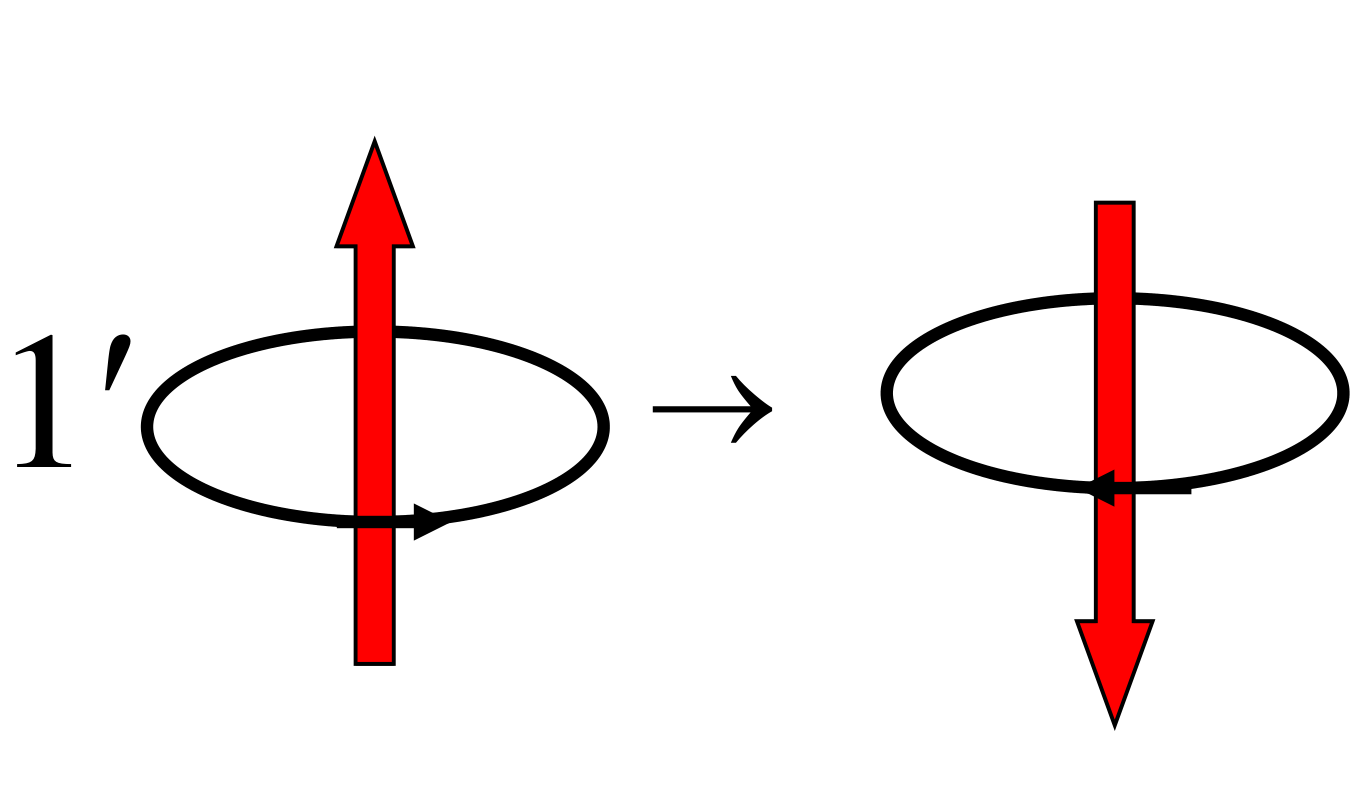
\includegraphics[height=0.6\linewidth]{fig/timerev.png}
  \caption{The time reversal operator $T = 1'$ reverses the electrical current, which inverts the magnetic moment.}
  \label{fig:timerev_a}
\end{subfigure} \hfill
\begin{subfigure}{.55\textwidth}
  \centering
  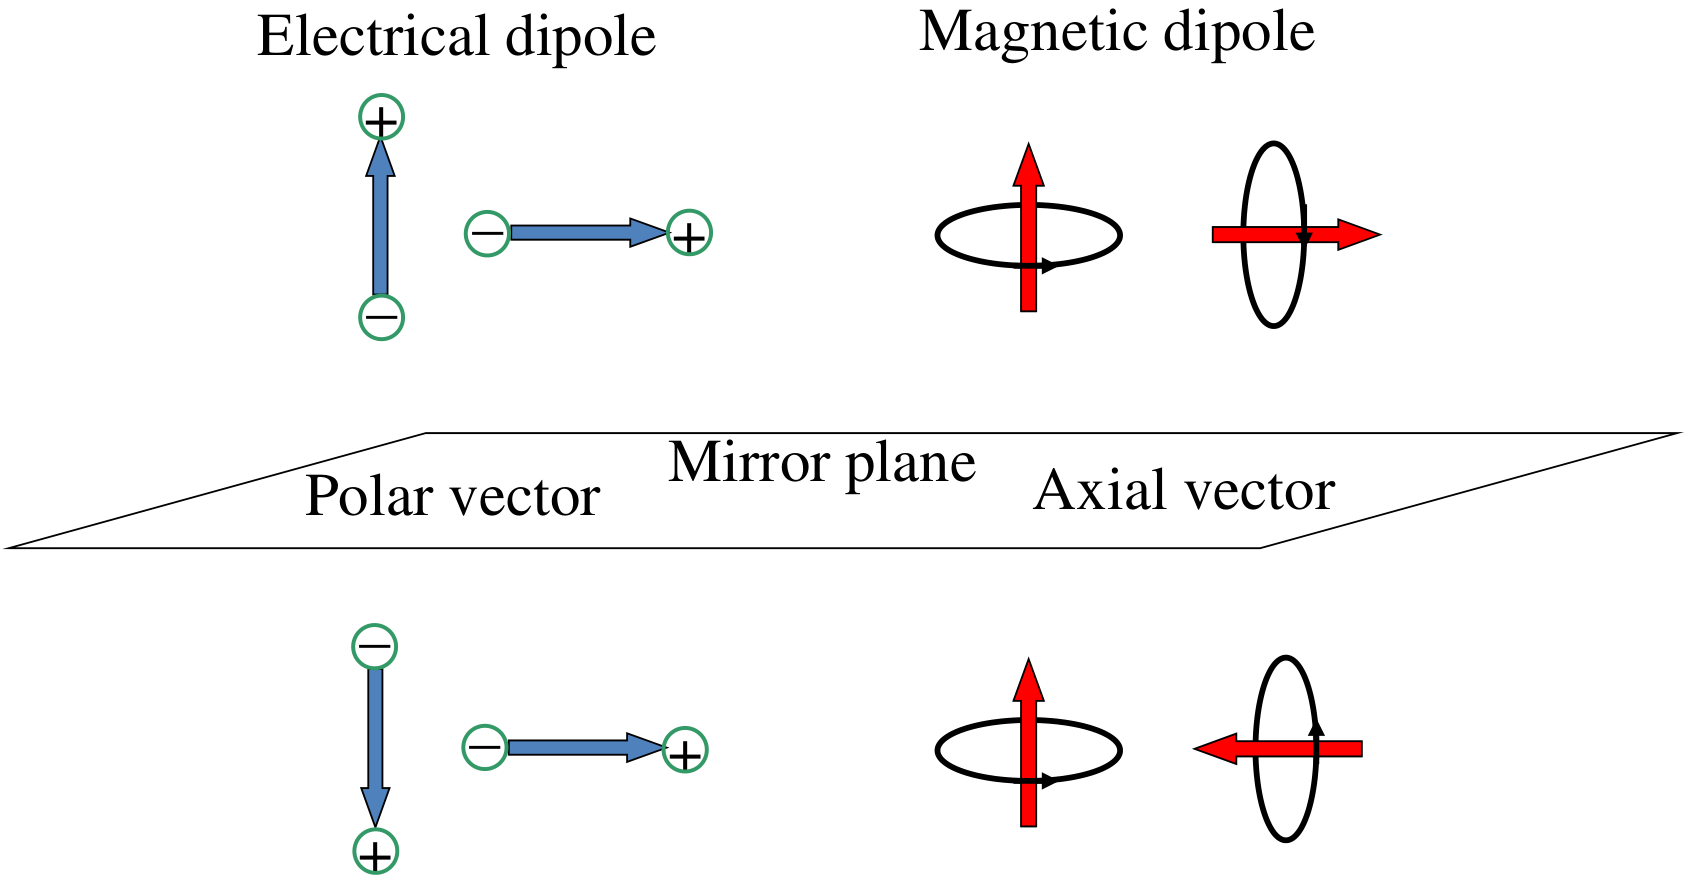
\includegraphics[width=\linewidth]{fig/axialvec.png}
  \caption{Comparison between a vector (electrical dipole) and an axial vector (magnetic dipole) under a reflection.}
  \label{fig:axialvec_b}
\end{subfigure}
\caption{The action of the time reversal operator. Figures taken from \cite{magnetic_structures2012}.}
\label{fig:timerev_axialvec}
\end{figure}

Although initially motivated by magnetic systems, the magnetic groups can be understood more abstractly as a mathematical construct: a tensor product with the group of two elements, \(\mathcal{T} = \{1, 1'\}\). In this view, time reversal is treated as an abstract operator, extending beyond its physical origins. %For instance, in the context of TBG, the time-reversal operator can be interpreted as \textbf{swapping the sublattice types \(A\) and \(B\) (ISSO ESTÁ ERRADOOOO, TALVEZ EU FALE DE TIME-REVERSAL IN SPINLESS SYSTEMS)}.

Let \(G\) be a group that does not include the time-reversal operator. A \textit{magnetic group} is then defined as a subgroup of the tensor product \(G \otimes \mathcal{T}\), where its elements can be ``painted black, white, or grey,'' reflecting the interplay between time-reversal and spatial symmetries.

\begin{definition}[\textbf{Magnetic group}] \label{def:magnetic_group}
Any magnetic group \( M \) can be expressed as a subgroup of the external direct product of \( \mathcal{T} = \{1, 1'\}\) with another group \( G \) (excluding \( 1' \)), such that \( M \subseteq G \otimes \mathcal{T} \). A magnetic group $M$ is defeined to be only one of three types:
\begin{enumerate}
\item \textbf{Colorless}: These are magnetic groups of the form \(M =  G \otimes \{1\} \).

\item \textbf{Grey (Paramagnetic)}: These are the full direct product \(M = G \otimes \{1, 1'\} \).

\item \textbf{Black-and-White}: If \( H \) is a subgroup of \( G \) with \hyperref[def:left_cosets]{index} \(2\), then \( M \) is constructed as
\begin{equation} \label{eq:magnetic_black_white_def}
M = H \otimes 1 \; \cup \; (G - H) \otimes 1'.
\end{equation}
\end{enumerate}
\end{definition}

\begin{figure}[H]
\centering
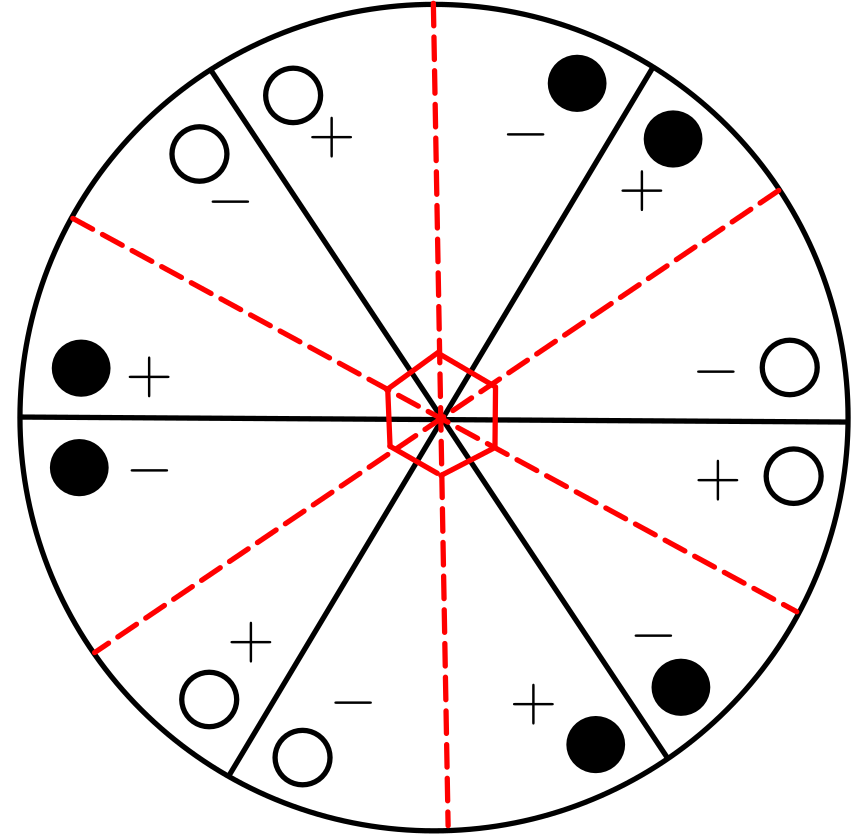
\includegraphics[width=0.5\linewidth]{fig/622_magnetic.png}
\caption{Representation of the magnetic point group $6'2'2$. \textbf{A FIGURA ESTÁ COM UM ERRO}, no South-East tá trocado $+$ e $-$.}
\label{fig:622_magnetic}
\end{figure}

\begin{example} \label{ex:magnetic_group_tbg_6'2'2}
The magnetic point group of the BM model of TBG is $6'2'2$ in Hermann-Mauguin notation. According to the notation, we can choose its generators to be $C_{6z} T$, $C_{2y} T$ and $C_{2x}$.
\end{example}

%%%%%%%%%%%%%%%%%%%%%%%%%%%%%%%%%%%%%%%%%%%%%%%%%%%%%%%%%%%%%%%%%%%%%%%%%%%%%%%%%%%%%%%%%%%%%%%%%%
\section{Topological Quantum Chemistry} \label{sec:topological_quantum_chemistry}
%%%%%%%%%%%%%%%%%%%%%%%%%%%%%%%%%%%%%%%%%%%%%%%%%%%%%%%%%%%%%%%%%%%%%%%%%%%%%%%%%%%%%%%%%%%%%%%%%%

%We are following the references \cite{lectures_tms2017, building_blocks2018}.

In this chapter we will introduce the formalism of Topological Quantum Chemistry (TQC) \cite{topological_quantum_chemistry2017, building_blocks2018, lectures_tms2017}. Among many things, this theory mathematically defines when a electronic band is topological, which is a concept intrinsically associated to the construction of Wannier orbitals for a tight-binding model. The application of these concepts play a major role to motivate and construct a fully symmetric interacting MATBG model.

%Since this theory involves numerous mathematical definitions and concepts, we will consistently use the example of monolayer graphene, which belongs to wallpaper group \#17 and the corresponding space group $P6mm$ ($\#183$ in international tables).

%\begin{figure}[H]
%\centering
%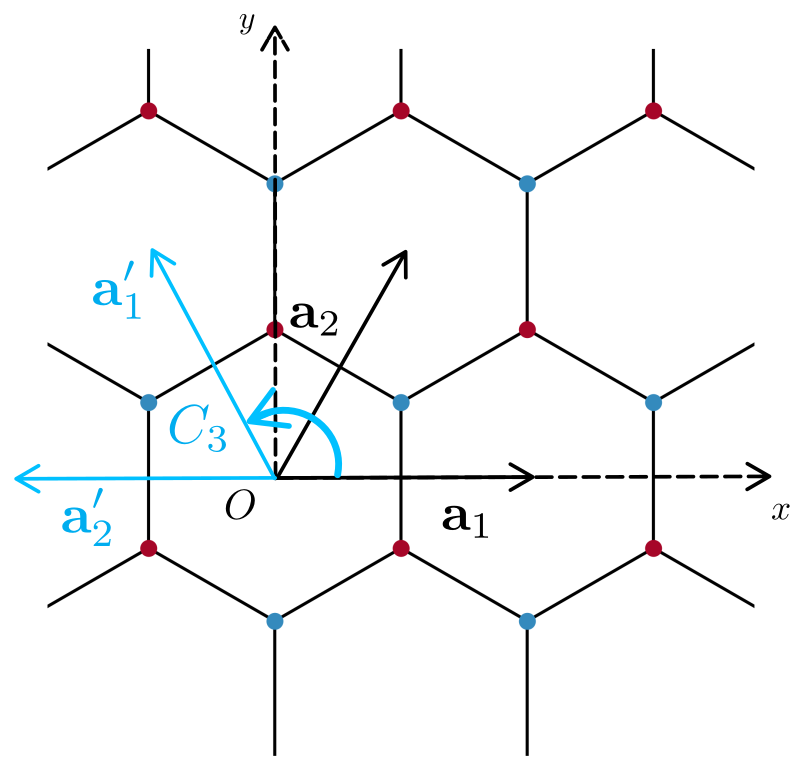
\includegraphics[width=0.32\linewidth]{fig/honeycomb_C3.png}\hfill
%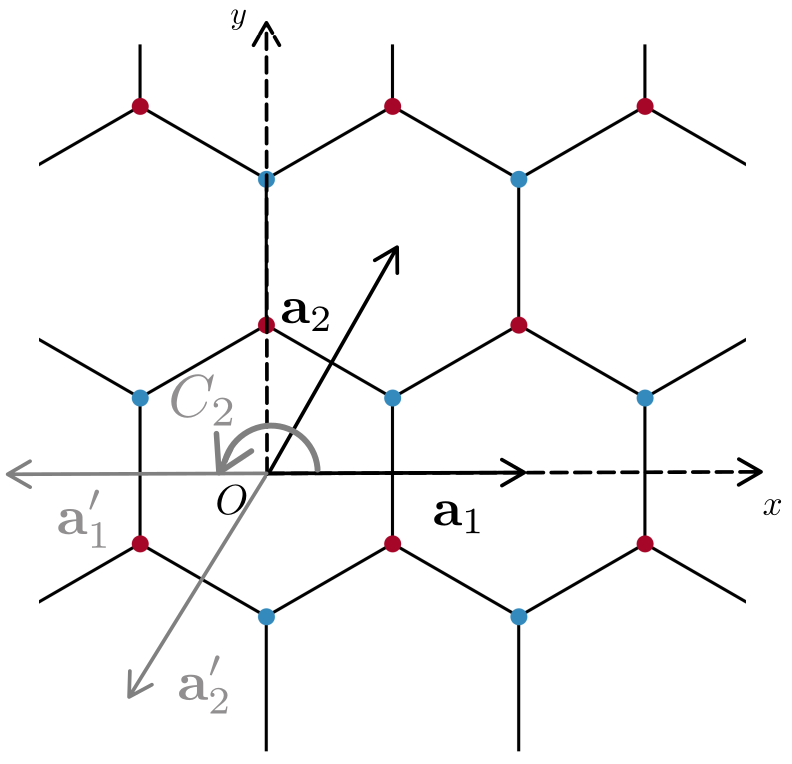
\includegraphics[width=0.32\linewidth]{fig/honeycomb_C2.png}\hfill
%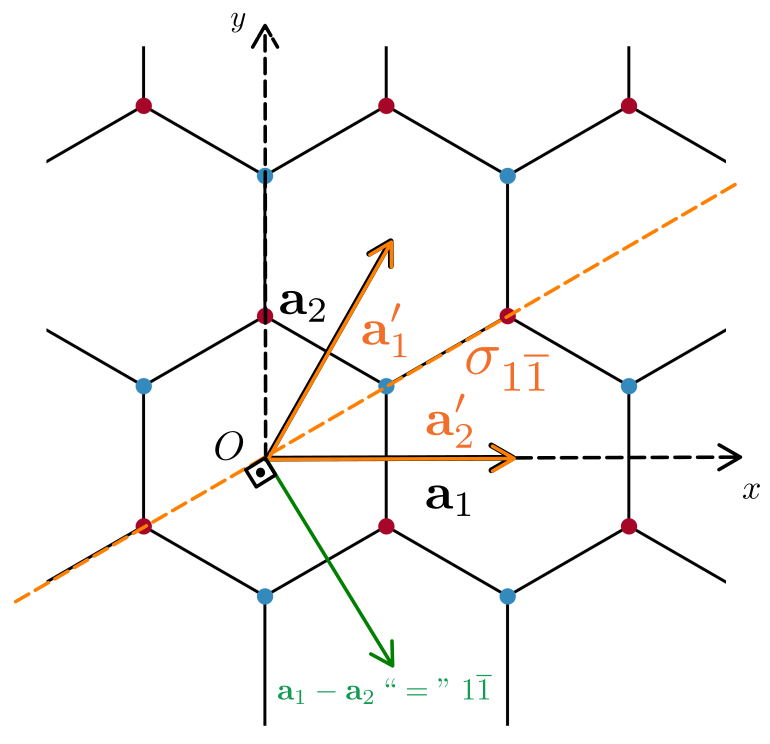
\includegraphics[width=0.32\linewidth]{fig/honeycomb_sigma.png}
%\caption{Generators of the point group \(\{C_3, C_2, m_{1\bar{1}}\}\) for the space group \(P6mm\) of the honeycomb lattice, with the coordinate system origin $O$ located at a hexagon's center. \textbf{CORRIGIR} $\sigma_{1\cc{1}} = m_{1\cc{1}}$.}
%\label{fig:generators_P6mm}
%\end{figure}
%
%Following Figure \ref{fig:generators_P6mm}, we use the basis $\mathcal{B} = \{\a_1 = a \vu{x}, \a_2 = \frac{a}{2} \vu{x} + \frac{a\sqrt{3}}{2} \vu{y}\}$. In this basis, the generators \(\{C_3, C_2, m_{1\bar{1}}\}\) for the point group $6mm$ act like:
%\begin{equation} \label{eq:generators_P6mm}
%\begin{cases}
%\; C_3 \a_1 = -\a_1+\a_2 \\
%\; C_3 \a_2 = -\a_1
%\end{cases}
%\quad
%\begin{cases}
%\; C_2\a_1 = -\a_1 \\
%\; C_2\a_2 = -\a_2
%\end{cases}
%\quad
%\begin{cases}
%\; m_{1\bar{1}} \a_1 = \a_2 \\
%\; m_{1\bar{1}} \a_2 = \a_1
%\end{cases}
%\end{equation}

%%%%%%%%%%%%%%%%%%%%%%%%%%%%%%%%%%%%%%%%%%%%%%%%%%%%%%%%%%%%%%%%%%%%%%%%%%%%%%%%%%%%%%%%%%%%%%%%%%
\subsection{Definitions} \label{subsec:tqc_definitions}
%%%%%%%%%%%%%%%%%%%%%%%%%%%%%%%%%%%%%%%%%%%%%%%%%%%%%%%%%%%%%%%%%%%%%%%%%%%%%%%%%%%%%%%%%%%%%%%%%%


\begin{definition}[\textbf{Orbit}] \label{def:orbit_q}
Given a point \(\q\), the \textit{orbit} of \(\q\) is the set of all points \textbf{within the same unit cell} that are related to \(\q\) by symmetry elements of the space group \(G\), i.e.,
\begin{equation} \label{eq:orbit_of_q}
\text{Orb}(\q) = G \q = \{g \q \mid g \in G\}.
\end{equation}
\end{definition}

%\begin{example} \label{ex:orbit_1a2b3c}
%In Figure \ref{fig:unitcell_q1q2q3q4q5}, using the basis $\mathcal{B} = \{\a_1, \a_2\}$, consider the points \(\textcolor{red}{\varhexagonblack} = \q_1 = (0,0)\), \(\textcolor{blue}{\mdblksquare} = \q_2 = \qty(\frac{1}{3}, \frac{1}{3})\), \(\textcolor{green}{\bigstar} = \q_3 = \qty(\frac{1}{2}, 0)\), \(\textcolor{magenta}{\varheartsuit} = \q_4 = \qty(\frac{1}{6}, \frac{1}{6})\), and \(\textcolor{orange}{\spadesuit} = \q_5 = \qty(\frac{1}{4}, 0)\).
%
%Note that the unit cell, as shown in Figure \ref{fig:unitcell_limit}, excludes points that are equivalent under translations by Bravais lattice vectors. By applying all symmetry elements of \(G\) to the points \(\q_1, \q_2, \q_3, \q_4, \q_5\) and retaining only those that lie within the same unit cell, the resulting orbits are represented by the symbols \(\textcolor{red}{\varhexagonblack}\), \(\textcolor{blue}{\mdblksquare}\), \(\textcolor{green}{\bigstar}\), \(\textcolor{magenta}{\varheartsuit}\), and \(\textcolor{orange}{\spadesuit}\), as shown in Figure \ref{fig:unitcell_orbitsymbols}.
%\end{example}
%
%\begin{figure}[H]
%\centering
%\begin{subfigure}{.3\textwidth}
%  \centering
%  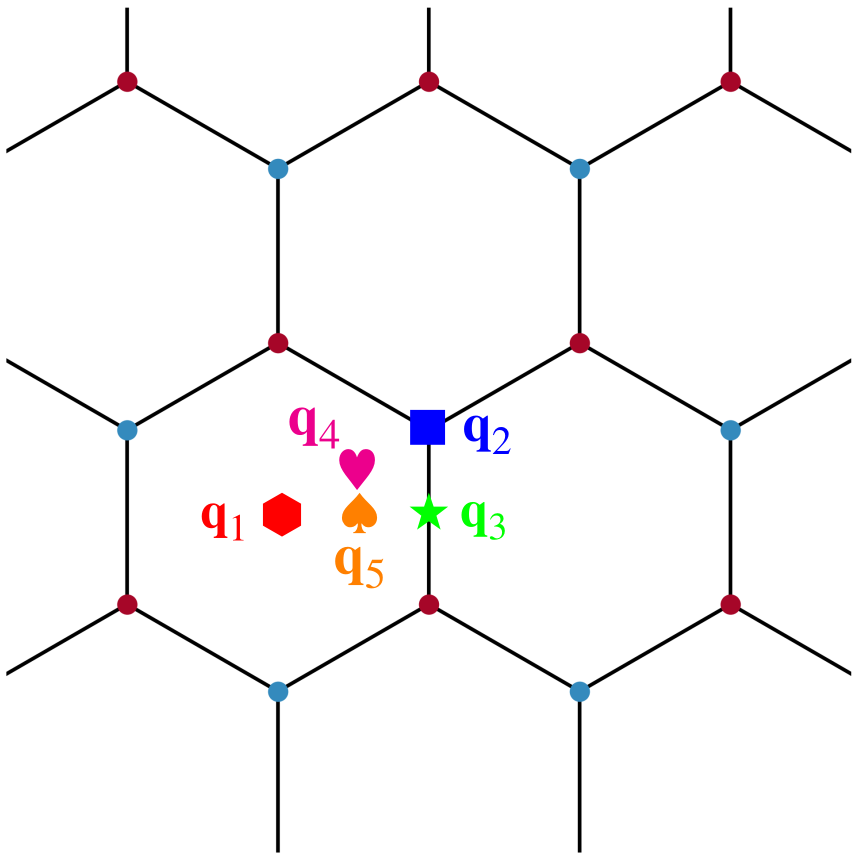
\includegraphics[width=\linewidth]{fig/unitcell_q1q2q3q4q5.png}
%  \caption{Points $\q_1,\q_2,\q_3,\q_4,\q_5$}
%  \label{fig:unitcell_q1q2q3q4q5}
%\end{subfigure}
%\hfill
%\begin{subfigure}{.3\textwidth}
%  \centering
%  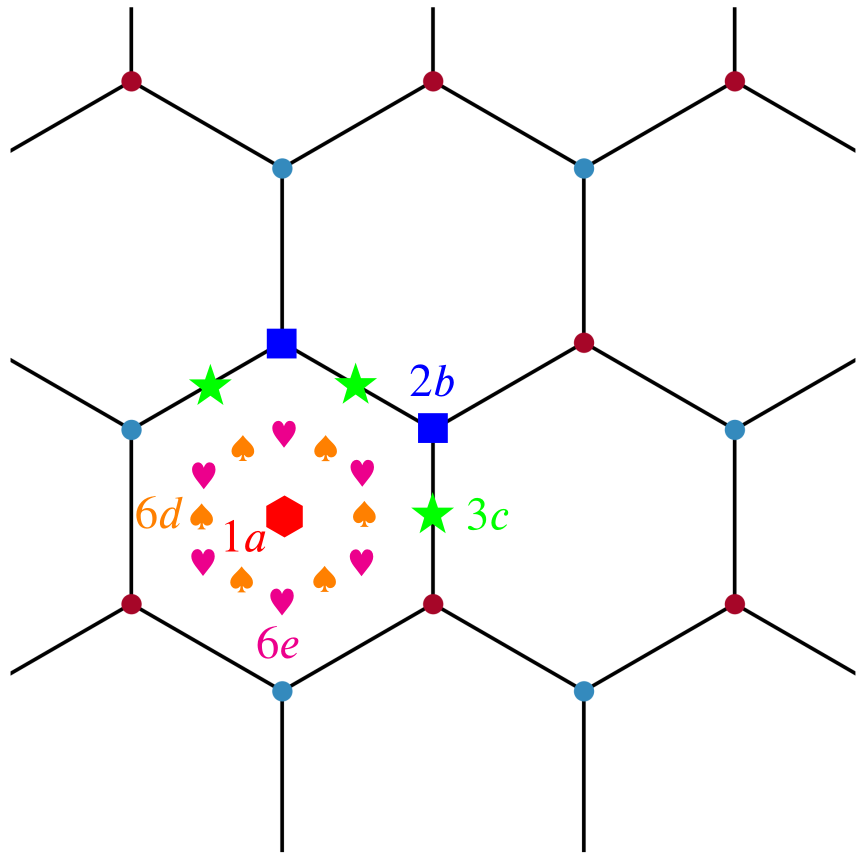
\includegraphics[width=\linewidth]{fig/unitcell_orbitsymbols.png}
%  \caption{Orbits and Wyckoff letters}
%  \label{fig:unitcell_orbitsymbols}
%\end{subfigure}
%\hfill
%\begin{subfigure}{.235\textwidth}
%  \centering
%  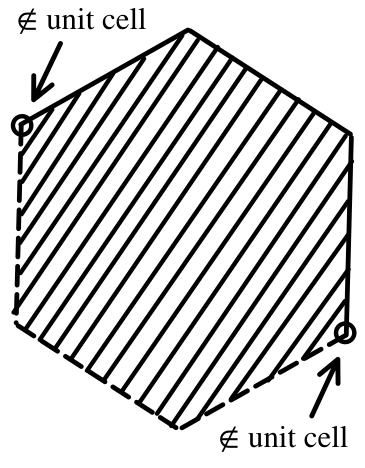
\includegraphics[width=\linewidth]{fig/unitcell_limit.png}
%  \caption{Unit cell choice}
%  \label{fig:unitcell_limit}
%\end{subfigure}
%\caption{Unit cell and orbits.}
%\label{fig:unitcell_orbits}
%\end{figure}


\begin{definition}[\textbf{Site-symmetry group / Stabilizer group}] \label{def:sitesym}
The site-symmetry group of a position $\q$ is the subgroup of operations $g \in G$ that leave $\q$ fixed.
\begin{equation} \label{eq:site-symmetry_def}
G_\q = \{g \mid g \q = \q\} \subseteq G.
\end{equation}
\end{definition}

%\textit{Remarks:}
%\begin{itemize}
%\item The site-symmetry group \( G_\q \) may include elements \(\{R \mid \r\}\) with \(\r \neq \0\).
%\item Since any site-symmetry group leaves a point invariant, it is isomorphic to one of the crystallographic point groups: $32$ in three dimensions and $10$ in two dimensions.
%\end{itemize}

%\begin{example} \label{ex:site-symmetry_groups_p6mm}
%Let us identify the site-symmetry groups of points $\q_1$, $\q_2$, $\q_3$, $\q_4$ and $\q_5$.
%
%\begin{itemize}
%\item The point $\textcolor{orange}{\spadesuit} = \q_5 = \qty(\frac{1}{4}, 0)$ has a site-symmetry group \(G_{\q_5}\) with only the identity $\{E \mid 0\}$ and $\{m_{x} \mid 0\}$ (reflection by the $x$-axis) as symmetry elements. This makes $G_{\q_5}$ isomorphic to $D_1$.
%\begin{equation} \label{eq:site-symmetry-q5}
%\{m_{x} \mid 0\} \q_3 = m_x \qty(\frac{1}{4} \a_1) = m_x \qty(\frac{a}{4} \vu{x}) = \frac{a}{4} \vu{x} = \frac{1}{4} \a_1 = \q_5.
%\end{equation}
%
%
%\item The point \(\textcolor{magenta}{\varheartsuit} = \q_4 = \qty(\frac{1}{6}, \frac{1}{6})\) has a site-symmetry group \(G_{\q_4}\) with only the identity $\{E \mid 0\}$ and $\{m_{1\cc{1}} \mid 0\}$ as symmetry elements. This also makes $G_{\q_4}$ isomorphic to $D_1$.
%\begin{align} \label{eq:site-symmetry-q4}
%\{m_{1\cc{1}} \mid 0\} \q_4 &= m_{1\cc{1}}\qty(\frac{1}{6} \a_1 + \frac{1}{6} \a_2) = \frac{1}{6} \a_2 + \frac{1}{6} \a_1 = \q_4.
%\end{align}
%
%\item The point \(\textcolor{green}{\bigstar} = \q_3 = \qty(\frac{1}{2}, 0)\) has a site-symmetry group \(G_{\q_3}\), which is isomorphic to \(D_2\). We can choose its generators to be $\{C_2 \mid \a_1\}$ and $\{m_{x}\mid 0\}$.
%\begin{align} \label{eq:site-symmetry-q3}
%\{C_2 \mid \a_1\} \q_3 &= C_2 \q_3 + \a_1 = -\q_3 + \a_1 = -\frac{1}{2} \a_1 + \a_1 = \q_3, \\
%\{m_{x} \mid 0\} \q_3 &= m_x \qty(\frac{1}{2} \a_1) = m_x \qty(\frac{a}{2} \vu{x}) = \frac{1}{2} \a_1 = \q_3.
%\end{align}
%
%\item The point $\textcolor{blue}{\mdblksquare} = \q_2 = \qty(\frac{1}{3}, \frac{1}{3})$ has site-symmetry group $G_{\q_2}$ isomorphic to $D_3$, and its generators are $\{C_3 \mid \a_1\}$ and $\{m_{1\cc{1}} \mid 0\}$.
%\begin{align} \label{eq:site-symmetry-q2}
%\{C_3 \mid \a_1\} \q_2 &= C_3 \qty(\frac{1}{3} \a_1 + \frac{1}{3} \a_2) + \a_1 = \frac{1}{3} \qty(-2\a_1 + \a_2) + \a_1 =
%\frac{1}{3} (\a_1 + \a_2) = \q_2, \\
%\{m_{1\cc{1}} \mid 0\} \q_2 &= m_{1\cc{1}} \qty(\frac{1}{3} \a_1 + \frac{1}{3} \a_2) =
%\frac{1}{3} \a_2 + \frac{1}{3} \a_1 = \q_2.
%\end{align}
%
%\item The point \(\textcolor{red}{\varhexagonblack} = \q_1 = (0,0)\) has a site-symmetry group \(G_{\q_1}\) isomorphic to \(D_6\), with generators \(\{C_3 \mid 0\}\), \(\{C_2 \mid 0\}\), and \(\{m_{1\cc{1}} \mid 0\}\). Since \(\q_1 = \0\) is the origin, it is evident that the action of any generator \(g\) on \(\q_1\) leaves it unchanged:
%\begin{equation} \label{eq:site-symmetry-q1}
%g \q_1 = \0 = \q_1, \quad \text{for all } g \in G_{\q_1}.
%\end{equation}
%\end{itemize}
%
%\end{example}

\begin{definition}[\textbf{Wyckoff position}] \label{def:wyckpos}
A \textit{Wyckoff position} \( \q \) refers to any position within the unit cell of the crystal. Some Wyckoff positions are \textit{special}, meaning they are left invariant by certain symmetry operations (other than the identity $\{E \mid 0\}$). The \textit{multiplicity} $n$ of a Wyckoff position is the number of distinct positions in its orbit within the same unit cell, $n = \abs{\text{Orb}(q)}$. A Wyckoff position is generally denoted as \( n\ell \), where \( \ell \) is an alphabetical label that designates the increasing size of the site-symmetry group associated with the position.
\end{definition}

%\begin{example} \label{ex:wyckpos_q1q2q3q4q5}
%The Wyckoff positions \( \q_1 = \textcolor{red}{\varhexagonblack} \), \( \q_2 = \textcolor{blue}{\mdblksquare} \), \( \q_3 = \textcolor{green}{\bigstar} \), \( \q_4 = \textcolor{magenta}{\varheartsuit} \), and \( \q_5 = \textcolor{orange}{\spadesuit} \) are respectively labeled as \( \textcolor{red}{1a} \), \( \textcolor{blue}{2b} \), \( \textcolor{green}{3c} \), \( \textcolor{magenta}{6d} \), and \( \textcolor{orange}{6e} \), as shown in Figure \ref{fig:unitcell_orbitsymbols}.
%\end{example}

\begin{definition}[\textbf{Coset representatives}] \label{def:cosetrep_wyckoff}
The \textit{coset representatives} of the site-symmetry group are the elements \( g_\alpha \) that generate the orbit of a Wyckoff position \( \q \), with each element in the orbit given by \( \q_\alpha = g_\alpha \q \). The number of coset representatives corresponds to the multiplicity of the Wyckoff position.
\end{definition}

%\begin{example} \label{ex:coset_representatives_q1q2q3q4q5}
%For the points $\q_1 = \textcolor{red}{\varhexagonblack}$, $\q_2 = \textcolor{blue}{\mdblksquare}$, $\q_3 = \textcolor{green}{\bigstar}$, $\q_4 = \textcolor{magenta}{\varheartsuit}$ and $\q_5 = \textcolor{orange}{\spadesuit}$, we can choose coset representatives as
%\begin{align}
%\text{Orb}(\q_1) &= \qty{\{E\mid 0\} \q_1}, \label{eq:orbit_q1} \\
%\text{Orb}(\q_2) &= \qty{\{E\mid 0\} \q_2, \{C_6\mid 0\} \q_2}, \label{eq:orbit_q2} \\
%\text{Orb}(\q_3) &= \qty{\{E\mid 0\} \q_3, \{C_6\mid 0\} \q_3, \{C_6^2\mid 0\} \q_3}, \label{eq:orbit_q3} \\
%\text{Orb}(\q_4) &= \qty{\{E\mid 0\} \q_4, \{C_6\mid 0\} \q_4, \{C_6^2\mid 0\} \q_4, \{C_6^3\mid 0\} \q_4, \{C_6^4\mid 0\} \q_4, \{C_6^5\mid 0\} \q_4}, \label{eq:orbit_q4} \\
%\text{Orb}(\q_5) &= \qty{\{E\mid 0\} \q_5, \{C_6\mid 0\} \q_5, \{C_6^2\mid 0\} \q_5, \{C_6^3\mid 0\} \q_5, \{C_6^4\mid 0\} \q_5, \{C_6^5\mid 0\} \q_5}, \label{eq:orbit_q5}
%\end{align}
%For example, in Equation \ref{eq:orbit_q3}, the coset representatives of $G_{\q_3}$ are $g_1 = \{E\mid 0\}$, $g_2 = \{C_6\mid 0\}$, and $g_3 = \{C_6^2\mid 0\}$.
%\end{example}

\begin{lemma}[\textbf{Coset decomposition}] \label{lemma:cosetdecomp_wyckoff}
Let \( \q \) be a Wyckoff position in a space group \( G \). The coset decomposition of \( G \) with respect to \( \q \) is given by:
\begin{equation} \label{eq:coset_decomp_wyckoff}
G = \bigcup_\alpha g_\alpha (G_{\q} \ltimes \Z^d),
\end{equation}
where \( \Z^d \) represents the group of lattice translations, \(\{E\mid \t\}\), with \(\t = \sum_{i=1}^d n_i \a_i\), where \( n_i \in \Z \) and \(\{\a_i\}\) are the primitive lattice vectors in \( d \) dimensions.

In practice, this decomposition means that for any \( g \in G \), we can write \( g = \{E \mid \t\} g_\alpha h \), for some translation \(\t\), coset representative \( g_\alpha \), and \( h \in G_\q \). Applying \( \q \) to both sides:
\begin{equation} \label{eq:coset_decomp_translation_t_step1}
g \q = \{E \mid \t\} g_\alpha h \q = \{E \mid \t\} g_\alpha \q = \{E \mid \t\} \q_\alpha = \q_\alpha + \t,
\end{equation}
which leads to
\begin{equation} \label{eq:coset_decomp_translation_t}
\t = g \q - \q_\alpha.
\end{equation}
\end{lemma}

%\begin{lemma}[\textbf{Conjugate site-symmetry groups}] \label{lemma:conjugate_group_G_qalpha}
%Positions \(\q\) and \(\q_\alpha\) on the same orbit are connected by the relation \(\q_\alpha = g_\alpha \q\), where \(g_\alpha\) is a coset representative. For \(h \in G_\q\), the following holds:
%\begin{equation} \label{eq:conjugate_group_qalpha}
%h \q = \q \implies h g_\alpha^{-1} \q_\alpha = g_\alpha^{-1} \q_\alpha \implies
%\qty(g_\alpha h g_\alpha^{-1}) \q_\alpha = \q_\alpha \implies
%g_\alpha h g_\alpha^{-1} \in G_{\q_\alpha}.
%\end{equation}
%Consequently, the site-symmetry groups of points on the same orbit are conjugates of each other, satisfying \(G_{\q_\alpha} = g_\alpha G_\q g_\alpha^{-1}\).
%\end{lemma}


%\begin{definition}[\textbf{Maximal Wyckoff position}] \label{def:maximal_wyckpos}
%A site-symmetry group is \textit{non-maximal} if there exists a finite group $H \neq G_\q$, such that $G_\q \subseteq H \subseteq G$. A site-symmetry group that is not non-maximal is \textit{maximal}. A Wyckoff position $\q$ is said to be \textit{maximal} if its site-symmetry group $G_\q$ is maximal.
%\end{definition}

%\begin{example} \label{ex:maximal_wyckpos_example}
%We have $G_{\q_4} \subset G_{\q_2}$ and $G_{\q_5} \subset G_{\q_3}$, therefore $\q_4$ and $\q_5$ are non-maximal Wyckoff positions. On the other hand, the Wyckoff positions $\q_1$, $\q_2$, $\q_3$ are maximal. \textbf{Do I prove this?}
%\end{example}

%%%%%%%%%%%%%%%%%%%%%%%%%%%%%%%%%%%%%%%%%%%%%%%%%%%%%%%%%%%%%%%%%%%%%%%%%%%%%%%%%%%%%%%%%%%%%%%%%%
\subsection{Band Representations} \label{subsec:band_reps}
%%%%%%%%%%%%%%%%%%%%%%%%%%%%%%%%%%%%%%%%%%%%%%%%%%%%%%%%%%%%%%%%%%%%%%%%%%%%%%%%%%%%%%%%%%%%%%%%%%

Consider a site \(\q\) within a Wyckoff position of multiplicity \(n\), hosting \(n_q\) orbitals. The corresponding wavefunctions, denoted as \(W_{i1}(\r)\) for \(i = 1, \ldots, n_q\), transform under an \(n_q\)-dimensional representation \(\rho\) of the site-symmetry group \(G_\q\):
\begin{equation} \label{eq:gWi1_nq_rep}
h W_{i1}(\r) = W_{i1}(h^{-1} \r) = \sum_{j} [\rho(h)]_{ij} W_{j1}(\r), \quad h \in G_\q.
\end{equation}

Without loss of generality, let the equivalent sites \(\q_\alpha = g_{\alpha} \q\) be in the same unit cell as \(\q\). The orbitals at \(\q_\alpha\) transform under the conjugate representation \(\rho_\alpha(h) = \rho(g_\alpha^{-1} h g_\alpha)\), where \(h \in G_{\q_\alpha}\) and \(g_\alpha^{-1} h g_\alpha \in G_\q\). The wavefunctions localized at \(\q_\alpha\) are then given by
\begin{equation} \label{eq:Wialpha_galpha_action}
W_{i\alpha}(\r) = g_\alpha W_{i1}(\r) = W_{i1}(g_\alpha^{-1} \r),
\end{equation}
where \(\alpha = 1, \ldots, n\) indexes the equivalent sites that belong to the Wyckoff position of multiplicity \(n\). The wavefunctions on other unit cells are obtained by applying a translation operator, such that:
\begin{equation} \label{eq:translated_Wialpha}
\sg{E}{\t_\mu} W_{i\alpha}(\r) = W_{i\alpha}(\r-\t_\mu),
\end{equation}
where $\t_\mu$ is a Bravais lattice vector.

There are \(n \times n_\q \times N\) wavefunctions \(W_{i\alpha}(\r - \t_\mu)\), where \(N \to \infty\) is the number of unit cells in the system. To determine their transformation properties under an arbitrary space group element \(g = \sg{R}{\t} \in G\), we derive the band representation \(\rho_G = \rho \uparrow G\) induced from the representation \(\rho\) of the site-symmetry group \(G_\q\), as in Definition \ref{def:induction_defi}.
\begin{equation} \label{eq:induced_rho_G_wannier_step1}
\rho_G(g) W_{i\alpha}(\r-\t_\mu) =
\underbrace{g \sg{E}{\t_\mu}}_{= \sg{E}{R\t_\mu} g} W_{i\alpha} (\r) =
\sg{E}{R\t_\mu} g W_{i\alpha} (\r) =
\sg{E}{R\t_\mu} \, (g g_\alpha) \, W_{i1} (\r).
\end{equation}

Applying Lemma \ref{lemma:cosetdecomp_wyckoff} for the element $g g_\alpha \in G$, we write $g g_\alpha = \sg{E}{\t_{\beta\alpha}} g_\beta h$, for some $h \in G_\q$, coset representative $g_\beta$ and a Bravais lattice vector $\t_{\beta\alpha}$ given by
\begin{equation} \label{eq:t_betaalpha}
\t_{\beta\alpha} = gg_\alpha \q - \q_\beta = g \q_\alpha - \q_\beta, \quad
h = g_\beta^{-1} \{E\mid -\t_{\beta\alpha}\} g g_\alpha.
\end{equation}

Following the derivation from Equation \ref{eq:induced_rho_G_wannier_step1}:
$$
\rho_G(g) W_{i\alpha}(\r-\t_\mu) =
\sg{E}{R\t_\mu} \qty(\sg{E}{\t_{\beta\alpha}} g_\beta h) W_{i1}(\r) =
\sg{E}{R\t_\mu + \t_{\beta\alpha}} g_\beta \sum_{j} [\rho(h)]_{ij} W_{j1}(\r) =
$$
$$
= \sum_{j} \sg{E}{R\t_\mu + \t_{\beta\alpha}} [\rho(h)]_{ij} W_{j\beta}(\r) \implies
$$
\begin{equation} \label{eq:wannier_rep}
\rho_G(g) W_{i\alpha}(\r-\t_\mu) = \sum_{j} [\rho(h)]_{ij} W_{j\beta}(\r - R\t_\mu - \t_{\beta\alpha}).
\end{equation}

\n

Now define the Bloch functions:
\begin{equation} \label{eq:bloch_functions}
a_{i\alpha}(\k, \r) = \sum_{\mu} e^{i\k\vdot\t_\mu} W_{i\alpha}(\r-\t_\mu).
\end{equation}

Using Equation \ref{eq:wannier_rep}, the Bloch functions transform as
$$
\rho_G(g) a_{i\alpha}(\k,\r) =
\rho_G(g) \sum_{\mu} e^{i\k\vdot\t_\mu} W_{i\alpha}(\r-\t_\mu) =
\sum_{j} \sum_{\mu} e^{i\k\vdot\t_\mu} [\rho(h)]_{ij} W_{j\beta}(\r-R\t_\mu-\t_{\beta\alpha}) =
$$
$$
= e^{-i(R\k)\vdot\t_{\beta\alpha}} \sum_{j} [\rho(h)]_{ji} \sum_{\mu} e^{i(R\k)\vdot(R\t_\mu+\t_{\beta\alpha})} W_{j\beta}(\r-R\t_\mu-\t_{\beta\alpha}) \implies
$$
\begin{equation} \label{eq:bloch_rep}
(\rho_G(g) a)_{i\alpha}(\k,\r) = e^{-i(R\k)\vdot\t_{\beta\alpha}} \sum_{j} [\rho(h)]_{ji} \, a_{j\beta}(R\k, \r),
\end{equation}
where $h$ and $\t_{\beta\alpha}$ are determined by Equation \ref{eq:t_betaalpha}. The choice of representatives $g_\alpha$ must be kept fixed through the construction.

Observe that $\rho_G(g)$ in its matrix form consists of infinitely many $(n\cdot n_q)\times (n\cdot n_q)$ block, where each one is labelled by a $(\k', \k)$ pair, that correspond to Bloch functions labelled by $\k', \k$. For a given $g = \sg{R}{\t} \in G$ and each set of columns corresponding to $\k$, there is exactly one non-zero block, identified by $\k' = R\k$. Denoting this block by $\rho_G^\k(g)$, its matrix elements are given by
$$
\qty[\rho_G^\k(g)]_{j\beta,i\alpha} = e^{-i(R\k)\vdot\t_{\beta\alpha}}\rho_{ij}(g_\beta^{-1}\sg{E}{-\t_{\beta\alpha}}gg_\alpha).
$$

The full set of matrices $\rho_G^\k(g)$, for each $\k$ in the first BZ, contain all the non-zero elements of $\rho_G(g)$.

%%%%%%%%%%%%%%%%%%%%%%%%%%%%%%%%%%%%%%%%%%%%%%%%%%%%%%%%%%%%%%%%%%%%%%%%%%%%%%%%%%%%%%%%%%%%%%%%%%%
%\subsection{Momentum space}
%%%%%%%%%%%%%%%%%%%%%%%%%%%%%%%%%%%%%%%%%%%%%%%%%%%%%%%%%%%%%%%%%%%%%%%%%%%%%%%%%%%%%%%%%%%%%%%%%%%

\begin{definition}[\textbf{Little group}]
Two reciprocal space vectors $\k_1$ and $\k_2$ are said to be equivalent, $\k_1 \equiv \k_2$, if $\k_2 - \k_1$ is a reciprocal lattice vector. The \textit{little group} $G_\k$ of a vector $\k$ in reciprocal space is the set of elements $g \in G$ such that $g \k \equiv \k$. Remember that the action of space group elements on reciprocal space is defined by
$$
g\k = \sg{R}{\t}\k = R\k.
$$
For each $\k$, notice that $G_\k$ is infinite because if $h \in G_\k$, the operation of $h$ followed by any Bravais lattice translation also belongs to $G_\k$.
\end{definition}

\n

The set \(\{\rho_G^\k(g) \mid g \in G_\k\}\) forms an \((n \cdot n_q) \times (n \cdot n_q)\) representation of the little group \(G_\k\), referred to as \(\rho_G \downarrow G_\k\). This subduction of \(\rho_G\) onto \(G_\k\) is projected onto the Wannier functions at \(\k\). Despite \(G_\k\) being infinite, the representations of two space group operations, \(\sg{R}{\t}\) and \(\sg{R}{\t + \t_1}\), where \(\t_1\) is a Bravais lattice translation, differ only by an overall phase factor \(e^{-i(R\k) \vdot \t_1} = e^{i\k \vdot \t_1}\) within \(\rho_G \downarrow G_\k\).

The characters of \(\rho_G^\k = \rho_G \downarrow G_\k\), analogous to the expression for induced representations' characters, are given for \(g \in G_\k\) as:

\begin{equation} \label{eq:}
\rho_G^\k(g) =
\sum_{\substack{\alpha=1 \\ g_\alpha^{-1}\sg{E}{-\t_{\alpha\alpha}}g g_\alpha \in G_\q}}^n e^{-i(R\k)\vdot\t_{\alpha\alpha}}
\chi^{(\rho)}\qty(g_\alpha^{-1}\sg{E}{-\t_{\alpha\alpha}}g g_\alpha),
\end{equation}
where \(\chi^{(\rho)}\) represents the character of the site-symmetry representation \(\rho\).

To determine the number of times each irrep \(\sigma_i^\k\) of \(G_\k\) appears in the representation \(\rho_G \downarrow G_\k\), denoted by \(r_i^\k\), we use the decomposition:

\begin{equation} \label{eq:induce_subduce}
(\rho \uparrow G) \downarrow G_\k \equiv \bigoplus_i r_i^\k \sigma_i^\k,
\end{equation}
where \(\equiv\) signifies the equivalence of representations. The multiplicities \(r_i^\k\) are computed using the \textit{Reduction Formula} \cite{dresselhaus}:

\begin{theorem}[\textbf{Reduction formula}] \label{th:reduction_formula}
Any unitary representation $\Gamma$ is a direct sum of irreps
\begin{equation} \label{eq:Gamma_direct_sum_of_irreps}
\Gamma \equiv \bigoplus_j r_j \, \Gamma_j,
\end{equation}
where the coefficients $r_j \in \N_{>0}$ denote the number of times the irrep $\Gamma_j$ appears in the decomposition of $\Gamma$. The coefficients $r_j$ are given by the \textit{reduction formula}
\begin{equation} \label{eq:reduction_formula}
r_j =
\frac{1}{\abs{G}} \sum_{g \in G} \chi^{(\Gamma)}(g) \chi^{(\Gamma_j)}(g)^* =
\frac{1}{\abs{G}} \sum_{S} \abs{S} \, \chi^{(\Gamma)}_S \qty[\chi^{(\Gamma_j)}_S]^*.
\end{equation}
\end{theorem}

%%%%%%%%%%%%%%%%%%%%%%%%%%%%%%%%%%%%%%%%%%%%%%%%%%%%%%%%%%%%%%%%%%%%%%%%%%%%%%%%%%%%%%%%%%%%%%%%%%
\subsection{Elementary Band Representations} \label{subsec:elementary_band_reps}
%%%%%%%%%%%%%%%%%%%%%%%%%%%%%%%%%%%%%%%%%%%%%%%%%%%%%%%%%%%%%%%%%%%%%%%%%%%%%%%%%%%%%%%%%%%%%%%%%%

Two band representations are considered equivalent if they can be continuously deformed into each other without closing energy gaps or breaking symmetries, similar to the concept of homotopy in topology. This notion of equivalence is essential for classifying electronic band structures in terms of their topological properties. By treating equivalence in this way, we can systematically identify whether a material exhibits non-trivial topological phases, such as those found in topological insulators, based purely on its symmetry and band structure.

\begin{definition}[\textbf{Equivalence between band representations}] \label{def:equiv_bandrep}
Two band representations $\rho_G$ and $\sigma_G$ are equivalent iff there exists a unitary matrix-valued function $S(\k,t,g)$ smooth in $\k$ and continuous in $t$ such that, for all $g \in G$
\begin{enumerate}
\item $S(\k, t, g)$ defines a band representation according to Equation \ref{eq:bloch_rep} for all $t \in [0,1]$;
\item $S(\k, 0, g) = \rho_G^\k(g)$;
\item $S(\k, 1, g) = \sigma_G^\k(g)$.
\end{enumerate}
\end{definition}

\begin{definition}[\textbf{Elementary band representation}]
A band representation is called \textbf{composite} if it is equivalent to the direct sum of other band representations. A band representation that is not composite is called \textbf{elementary}.
\end{definition}

%\begin{theorem}[\textbf{Properties of band representations}]
%Some properties of band representations are:
%\begin{enumerate}
%\item Because induction commutes with direct sums
%$$
%(\rho_1 \oplus \rho_2) \uparrow G = (\rho_1 \uparrow G) \oplus (\rho_2 \uparrow G),
%$$
%reducible representations of $G_\q$ induce composite band representations.
%
%\item Given subgroups $K \subset H \subset G$, and a representation $\rho$ of $K$, because induction is transitive it follows that
%$$
%(\rho \uparrow H) \uparrow G = \rho \uparrow G.
%$$
%From this we conclude that all EBRs can be induced from irreps of the maximal site symmetry groups.
%\end{enumerate}
%\end{theorem}

%%%%%%%%%%%%%%%%%%%%%%%%%%%%%%%%%%%%%%%%%%%%%%%%%%%%%%%%%%%%%%%%%%%%%%%%%%%%%%%%%%%%%%%%%%%%%%%%%%%
%\subsection{Exceptions}
%%%%%%%%%%%%%%%%%%%%%%%%%%%%%%%%%%%%%%%%%%%%%%%%%%%%%%%%%%%%%%%%%%%%%%%%%%%%%%%%%%%%%%%%%%%%%%%%%%%
%
%There are exceptions where an irrep of the site symmetry group of a maximal Wyckoff position induces a composite band representation.

%%%%%%%%%%%%%%%%%%%%%%%%%%%%%%%%%%%%%%%%%%%%%%%%%%%%%%%%%%%%%%%%%%%%%%%%%%%%%%%%%%%%%%%%%%%%%%%%%%
\subsection{Topological Systems} \label{subsec:topological_systems}
%%%%%%%%%%%%%%%%%%%%%%%%%%%%%%%%%%%%%%%%%%%%%%%%%%%%%%%%%%%%%%%%%%%%%%%%%%%%%%%%%%%%%%%%%%%%%%%%%%

The \textit{atomic limit} refers to bands that can be constructed from localized orbitals situated on atomic sites while fully preserving the crystal's symmetry. These bands represent tightly bound electrons and lack any global topological properties. In contrast, \textit{topological bands} cannot be derived from such localized orbitals without violating symmetry or continuity. Their wavefunctions exhibit a global ``twisting'' that fundamentally sets them apart from the atomic case. Based on this concept, we define the following \cite{building_blocks2018}:

\begin{definition}[\textbf{Topological band}]
A set of bands are in the \textbf{atomic limit} of a space group if they can be induced from localized Wannier functions consistent with the crystalline symmetry of that space group. Otherwise, they are \textbf{topological}.
\end{definition}

Band representations describe systems in the atomic limit, where bands can be derived from localized Wannier orbitals that respect the crystal's symmetry. In contrast, topological bands are groups of bands that adhere to the crystal symmetry in momentum space but cannot be expressed as a band representation. This means they cannot be induced from symmetry-preserving localized Wannier orbitals. This inability is referred to as a \textit{Wannier obstruction} \cite{FragileTopology_Po2018, building_blocks2018}.

\begin{theorem} \label{th:topo_insul}
Any isolated set of bands that is not equivalent to a band representation (composite or elementary) gives a strong, weak, or crystalline topological insulator.
\end{theorem}


%%%%%%%%%%%%%%%%%%%%%%%%%%%%%%%%%%%%%%%%%%%%%%%%%%%%%%%%%%%%%%%%%%%%%%%%%%%%%%%%%%%%%%%%%%%%%%%%%%%
%\subsection{How to determine if a set of bands is topological}
%%%%%%%%%%%%%%%%%%%%%%%%%%%%%%%%%%%%%%%%%%%%%%%%%%%%%%%%%%%%%%%%%%%%%%%%%%%%%%%%%%%%%%%%%%%%%%%%%%%
%
%As said in \cite{building_blocks2018}: \textbf{ESSA SEÇÃO EU COPIEI}
%
%A practical route to determining whether a set of bands $\mathcal{B}$ is \textbf{not} a band representation is as follows: first, enumerate all EBRs for the particular space group and list the irreps that appear in each EBR at each high symmetry point. Next, compute the irreps at each high-symmetry point for the bands in $\mathcal{B}$. If the set of irreps that have been computed for the bands in $\mathcal{B}$ cannot be obtained from a linear combination of the EBRs in the space group, then the bands in $\mathcal{B}$ do not comprise a band representation and, by Theorem \ref{th:topo_insul}, are topological.
%
%If the irreps that appear in $\mathcal{B}$ can be obtained from a linear combination of the EBRs of the space group, then one must compute symmetric and localized Wannier functions for the bands in $\mathcal{B}$ to confirm that they are equivalent to the atomic limit defined by the linear combination of EBRs or compute a Berry phase that will distinguish the two. This is because, it is possible for two distinct groups of bands to have the exact same irreps at all high-symmetry points, but different Berry phases (recall, this is exactly why we require the homotopic notion of equivalence, as in Definition \ref{def:equiv_bandrep}.)


To determine whether a set of bands \(\mathcal{B}\) does \textbf{not} form a band representation, a systematic approach can be followed: first, identify all elementary band representations (EBRs) for the relevant space group and catalog the irreducible representations (irreps) that appear at each high-symmetry point for these EBRs. Then, calculate the irreps associated with the bands in \(\mathcal{B}\) at the high-symmetry points. If the irreps corresponding to \(\mathcal{B}\) cannot be expressed as a linear combination of the irreps from the EBRs, the bands do not form a band representation. According to Theorem \ref{th:topo_insul}, this indicates that the bands are topological.

If the irreps of \(\mathcal{B}\) can be written as a linear combination of EBRs, further analysis is required. One must either construct symmetric, localized Wannier functions to verify that the bands correspond to the atomic limit implied by the linear combination of EBRs, or calculate a Berry phase to distinguish between the two cases. This additional step is necessary because distinct sets of bands can share identical irreps at all high-symmetry points while differing in their Berry phases, reflecting the need for the homotopic equivalence notion described in Definition \ref{def:equiv_bandrep}.



%%%%%%%%%%%%%%%%%%%%%%%%%%%%%%%%%%%%%%%%%%%%%%%%%%%%%%%%%%%%%%%%%%%%%%%%%%%%%%%%%%%%%%%%%%%%%%%%%%
\section{Topological Heavy Fermion Model} \label{sec:topo_heavy_fermion}
%%%%%%%%%%%%%%%%%%%%%%%%%%%%%%%%%%%%%%%%%%%%%%%%%%%%%%%%%%%%%%%%%%%%%%%%%%%%%%%%%%%%%%%%%%%%%%%%%%

The representations and Elementary Band Representations (EBRs) for a given (magnetic) space group, such as \( P6'2'2 \), can be conveniently obtained from the Bilbao Crystallographic Server \cite{bilbao_1, bilbao_2}.

\begin{table}[H]
\caption{Character table of irreps at high symmetry momenta in magnetic space group $P6'2'2$.}
\centering
\begin{tabular} { c c c c | c c c | c c c }
\cline{1-10}
$\P$ & $\P \Gamma_1$ & $\P \Gamma_2$ & $\P \Gamma_3$ & $\P$ & $\P M_1$ & $\P M_2$ & $\P$ & $\P K_1$ & $\P K_2K_3$ \\
\cline{1-10}
$E$ & $\P1$ & $\P1$ & $\P2$ & $\P E$ & $\P1$ & $\P1$ & $\P E$ & $\P1$ & $\P2$ \\
$2 C_3$ & $\P1$ & $\P1$ & $ -1$ & $\P C_2'$ & $\P1$ & $ -1$ & $\P C_3$ & $\P1$ & $ -1$ \\
$3 C_2'$ & $\P1$ & $ -1$ & $\P0$ & $\P$ & $\P$ & $\P$ & $\P C_3^{-1}$ & $\P1$ & $-1$ \\
\cline{1-10}
\end{tabular}
\label{tab:P6'2'2}
\end{table}

\begin{table}[H]
\footnotesize
\caption{Elementary band representations of the magnetic space group $P6'2'2$.}
\centering
\begin{tabular}{|c|c|c|c|c|c|c|c|c|}
\hline
Wyckoff & \multicolumn{3}{c|}{$1a$} & \multicolumn{3}{c|}{$2c$} & \multicolumn{2}{c|}{$3f$} \\
\cline{1-9}
Site sym. & \multicolumn{3}{c|}{$6'2'2$, $32$} & \multicolumn{3}{c|}{$32$, $32$} & \multicolumn{2}{c|}{$2'2'2$, $2$} \\
\cline{1-9}
EBR & $G_{A_1}^{1a}(1)$ & $G_{A_2}^{1a}(1)$ & $G_{E}^{1a}(2)$ & $G_{A_1}^{2c}(2)$ & $G_{A_2}^{2c}(2)$ & $G_{E}^{2c}(4)$   & $G_{A}^{3f}(3)$ & $G_{B}^{3f}(3)$ \\
\hline
$\Gamma$ & $\Gamma_1$ & $\Gamma_2$ & $\Gamma_3$ & $2\Gamma_1$ & $2\Gamma_2$ & $2\Gamma_3$ & $\Gamma_1+\Gamma_3$ & $\Gamma_2+\Gamma_3$ \\
\hline
$K$ & $K_1$ & $K_1$ & $K_2 K_3$ & $K_2 K_3$ & $K_2 K_3$ & $2K_1 + K_2 K_3$ & $K_1+K_2 K_3$ & $K_1+K_2 K_3$ \\
\hline
$M$ & $M_1$ & $M_2$ & $M_1+M_2$ & $2M_1$ & $2M_2$ & $2M_1+2M_2$ & $2M_1+M_2$ & $M_1+2M_2$ \\
\hline
\end{tabular}
\label{tab:matbg-irreps}
\end{table}

As demonstrated in \cite{all_magic_angles}, incorporating the emergent particle-hole symmetry within the One Valley BM model ensures that the middle two flat bands in each valley align with the irreducible co-representations (irreps):
\begin{equation} \label{eq:matbg-irreps}
\Gamma_1(1) \oplus \Gamma_2(1); \; M_1(1) \oplus M_2(1); \; K_2 K_3(2),
\end{equation}
associated with the magnetic space group \( P6'2'2 \). The characters for each of these irreps, referenced in Equation \ref{eq:matbg-irreps}, are presented in Table \ref{tab:P6'2'2}.


By comparing the irreps in Equation \ref{eq:matbg-irreps} with the EBRs in Table \ref{tab:matbg-irreps}, we observe that the irreps in Equation \ref{eq:matbg-irreps} cannot be expressed as a direct sum of the local orbitals listed in Table \ref{tab:matbg-irreps}. In fact, if we permit negative coefficients, the irreps can only be expressed as the linear combination \( G_{A_1}^{2c} + G_{A_2}^{1a} - G_{A_1}^{1a} \). The presence of a negative coefficient indicates that the two flat bands must host at least a fragile topological phase \cite{FragileTopology_Po2018}, leading to a Wannier obstruction.

To resolve this Wannier obstruction, we incorporate the nearest higher-energy bands, which are characterized by the \(\Gamma_3\) irrep at the \(\Gamma_M\) point \cite{topoheavyfermion2022}. These higher-energy bands hybridize with the two middle bands, allowing us to isolate the trivial bands. These trivial bands form the band representation:
\begin{equation} \label{eq:trivial-irreps}
G_E^{1a}(2) = [E]_{1a} \uparrow G: \quad \Gamma_3(2); \; M_1(1) \oplus M_2(1); \; K_2 K_3(2),
\end{equation}
where \([E]_{1a}\) corresponds to \(p_x \pm i p_y\)-like orbitals at the \(1a\) Wyckoff position.

We ``borrow'' a $\Gamma_3$ irrep from these higher-energy bands to replace the $\Gamma_1 \oplus \Gamma_2$ states. The resulting irreps $\Gamma_3$, $M_1 \oplus M_2$, $K_2 K_3$ are consistent with $p_x \pm i p_y$ orbitals on a triangular lattice. To model this, Gaussian Wannier functions (WFs) that transform as $p_x \pm i p_y$ under the crystal symmetries are introduced.

Using the maximal localization procedure \cite{maxlocalWFs_marzari2012, wannier90}, we find that these WFs are highly localized, supported by flat band states away from $\Gamma_M$, and by low-energy states near $\Gamma_M$. However, to fully account for the superconducting properties, it is crucial to include the remaining states. To achieve this, we define projectors $\bP$ (onto the WFs) and $\I$ (onto the lowest six bands per spin-valley), and decompose the BM Hamiltonian $H_\text{BM}$ into the following components:
\begin{equation} \label{eq:projected_hamiltonians_WFs_PQ}
H^{(f)} = \bP H_\text{BM} \bP, \quad H^{(c)} = \bQ H_\text{BM} \bQ, \quad H^{(fc)} = \bP H_\text{BM} \bQ, \quad H^{(cf)} = H^{(fc)\dagger},
\end{equation}
where $\bQ = \I - \bP$. Since the coupling between WFs is extremely weak, the approximation $H^{(f)} \approx 0$ proves to be highly accurate.

The two states in $\bP$ form $\Gamma_3$ at $\Gamma_M$, while the four states in $\bQ$ form $\Gamma_3 \oplus \Gamma_1 \oplus \Gamma_2$. The remaining Hamiltonian $H^{(c)}$ in valley $\eta$ is expressed as:
\begin{equation} \label{eq:H(c)_topoheavyfermion}
H^{(c, \eta)}(\k) =
\begin{pmatrix}
0_{2\times 2} & v_* (\eta k_x \sigma_0 + i k_y \sigma_z) \\
v_* (\eta k_x \sigma_0 - i k_y \sigma_z) & M \sigma_x
\end{pmatrix}.
\end{equation}

The coupling $H^{(fc)}$ takes the form:
\begin{equation} \label{eq:H(fc)_topoheavyfermion}
H^{(fc, \eta)}(\k) =
\begin{pmatrix}
\gamma \sigma_0 + v'_* (\eta k_x \sigma_x + k_y \sigma_y) & 0_{2\times 2}
\end{pmatrix},
\end{equation}
which introduces a gap in $H^{(c, \eta)}$, establishing the flat band topology of the BM model.

Using standard parameters for MATBG, this mapping provides the parameter values:
\begin{equation} \label{eq:paramaters_topoheavyfermion}
v^\star = -4.303 \, \text{eV} \cdot \AA, \quad M = 3.697 \, \text{meV}, \quad \gamma = -24.75 \, \text{meV}, \quad v'^\star = 1.622 \, \text{eV} \cdot \AA.
\end{equation}

By diagonalizing the resulting 6-band model for the valley $\eta = +$, constructed from the Hamiltonians $H^{(c,\eta)}$ and $H^{(fc,\eta)}$, we obtain the results shown in Figure \ref{fig:thf-exploration}. We analyze the cases where certain parameters are set to zero to study the model's behavior.

\begin{figure}[H]
\centering
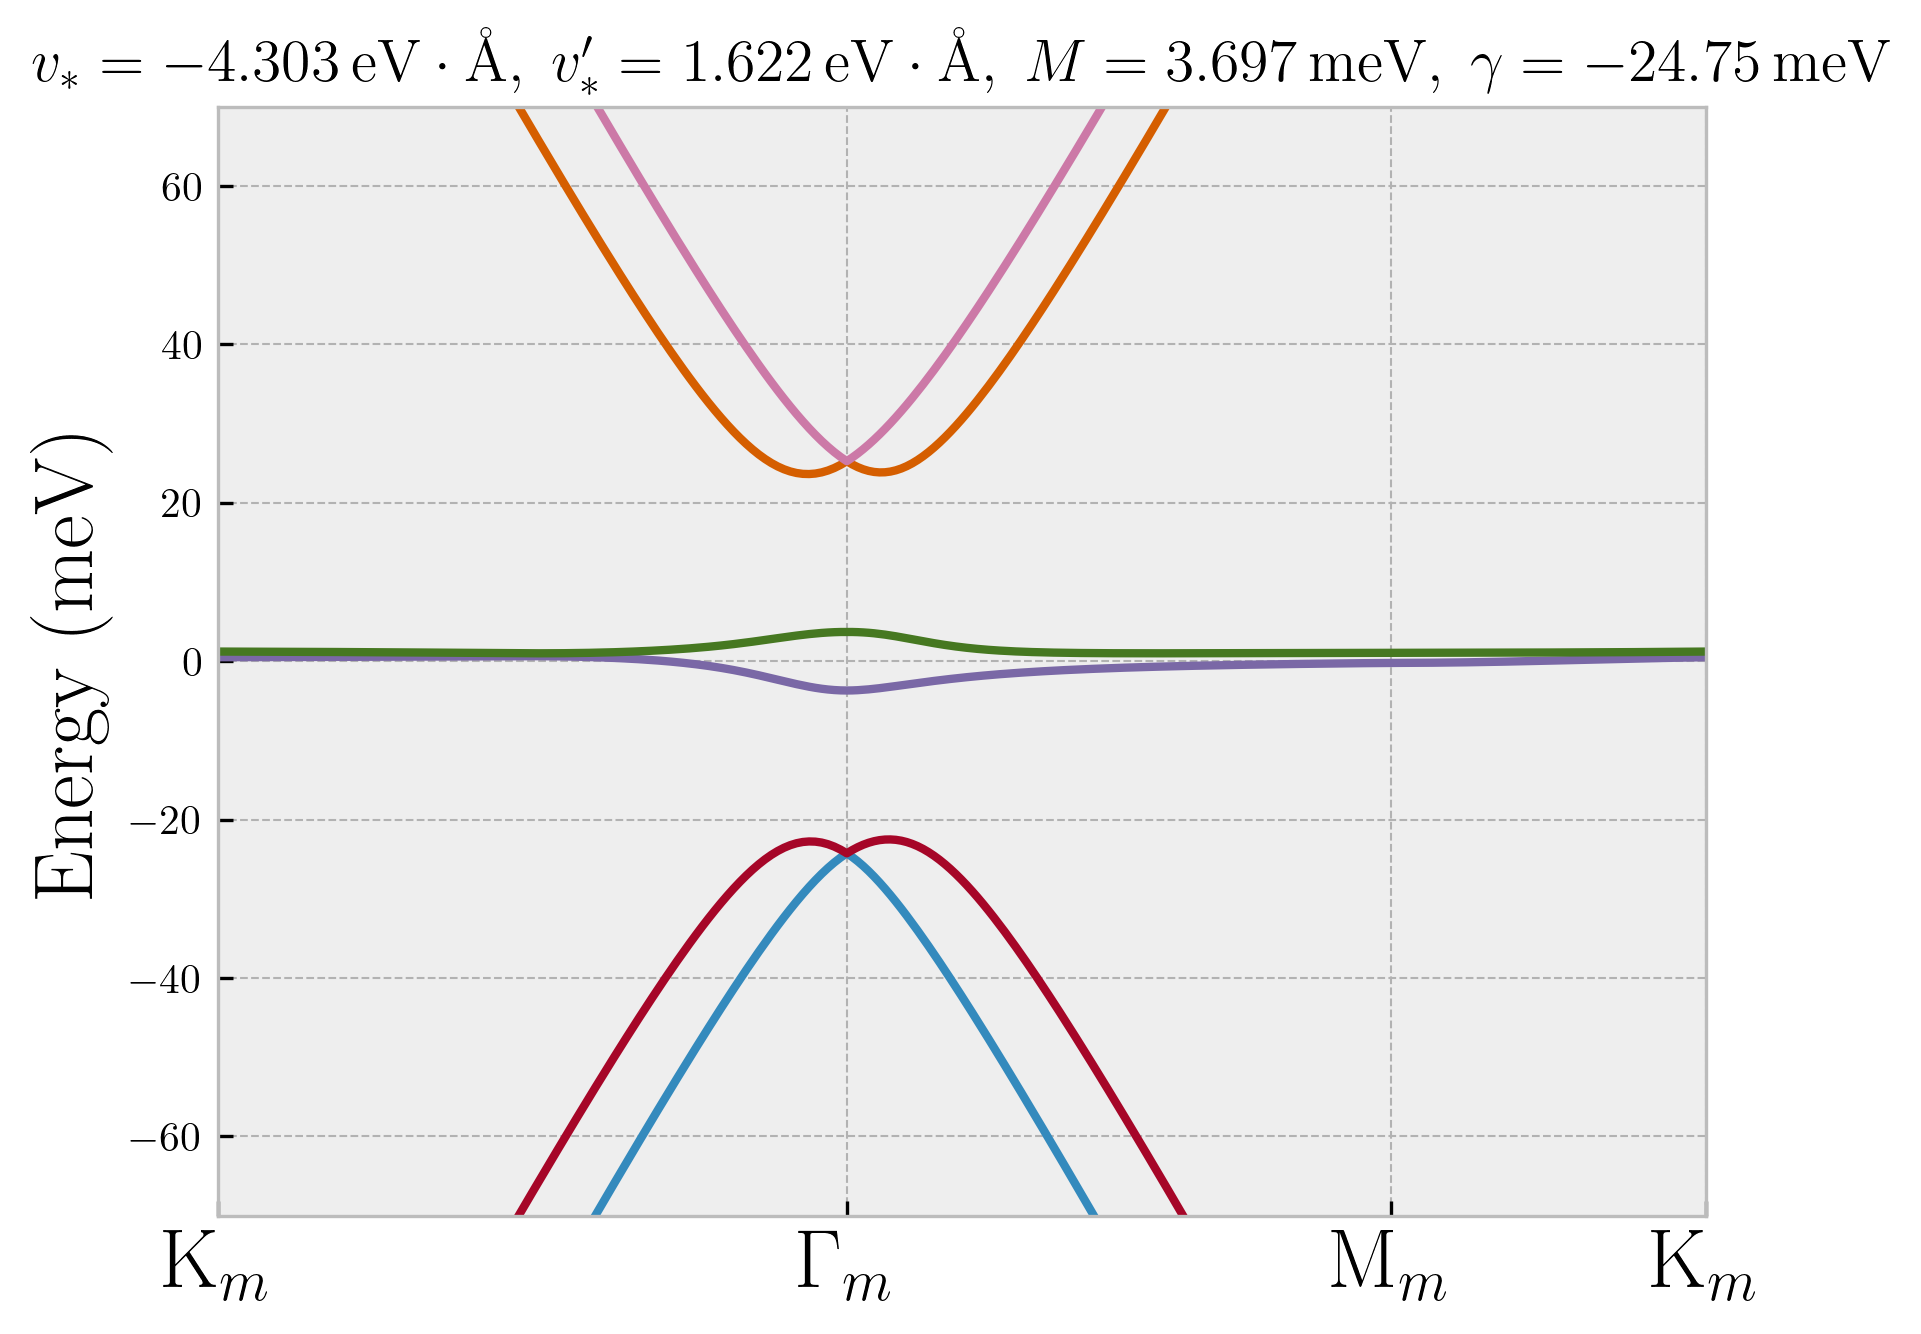
\includegraphics[height=0.35\linewidth]{fig/thf-correct_params.png}
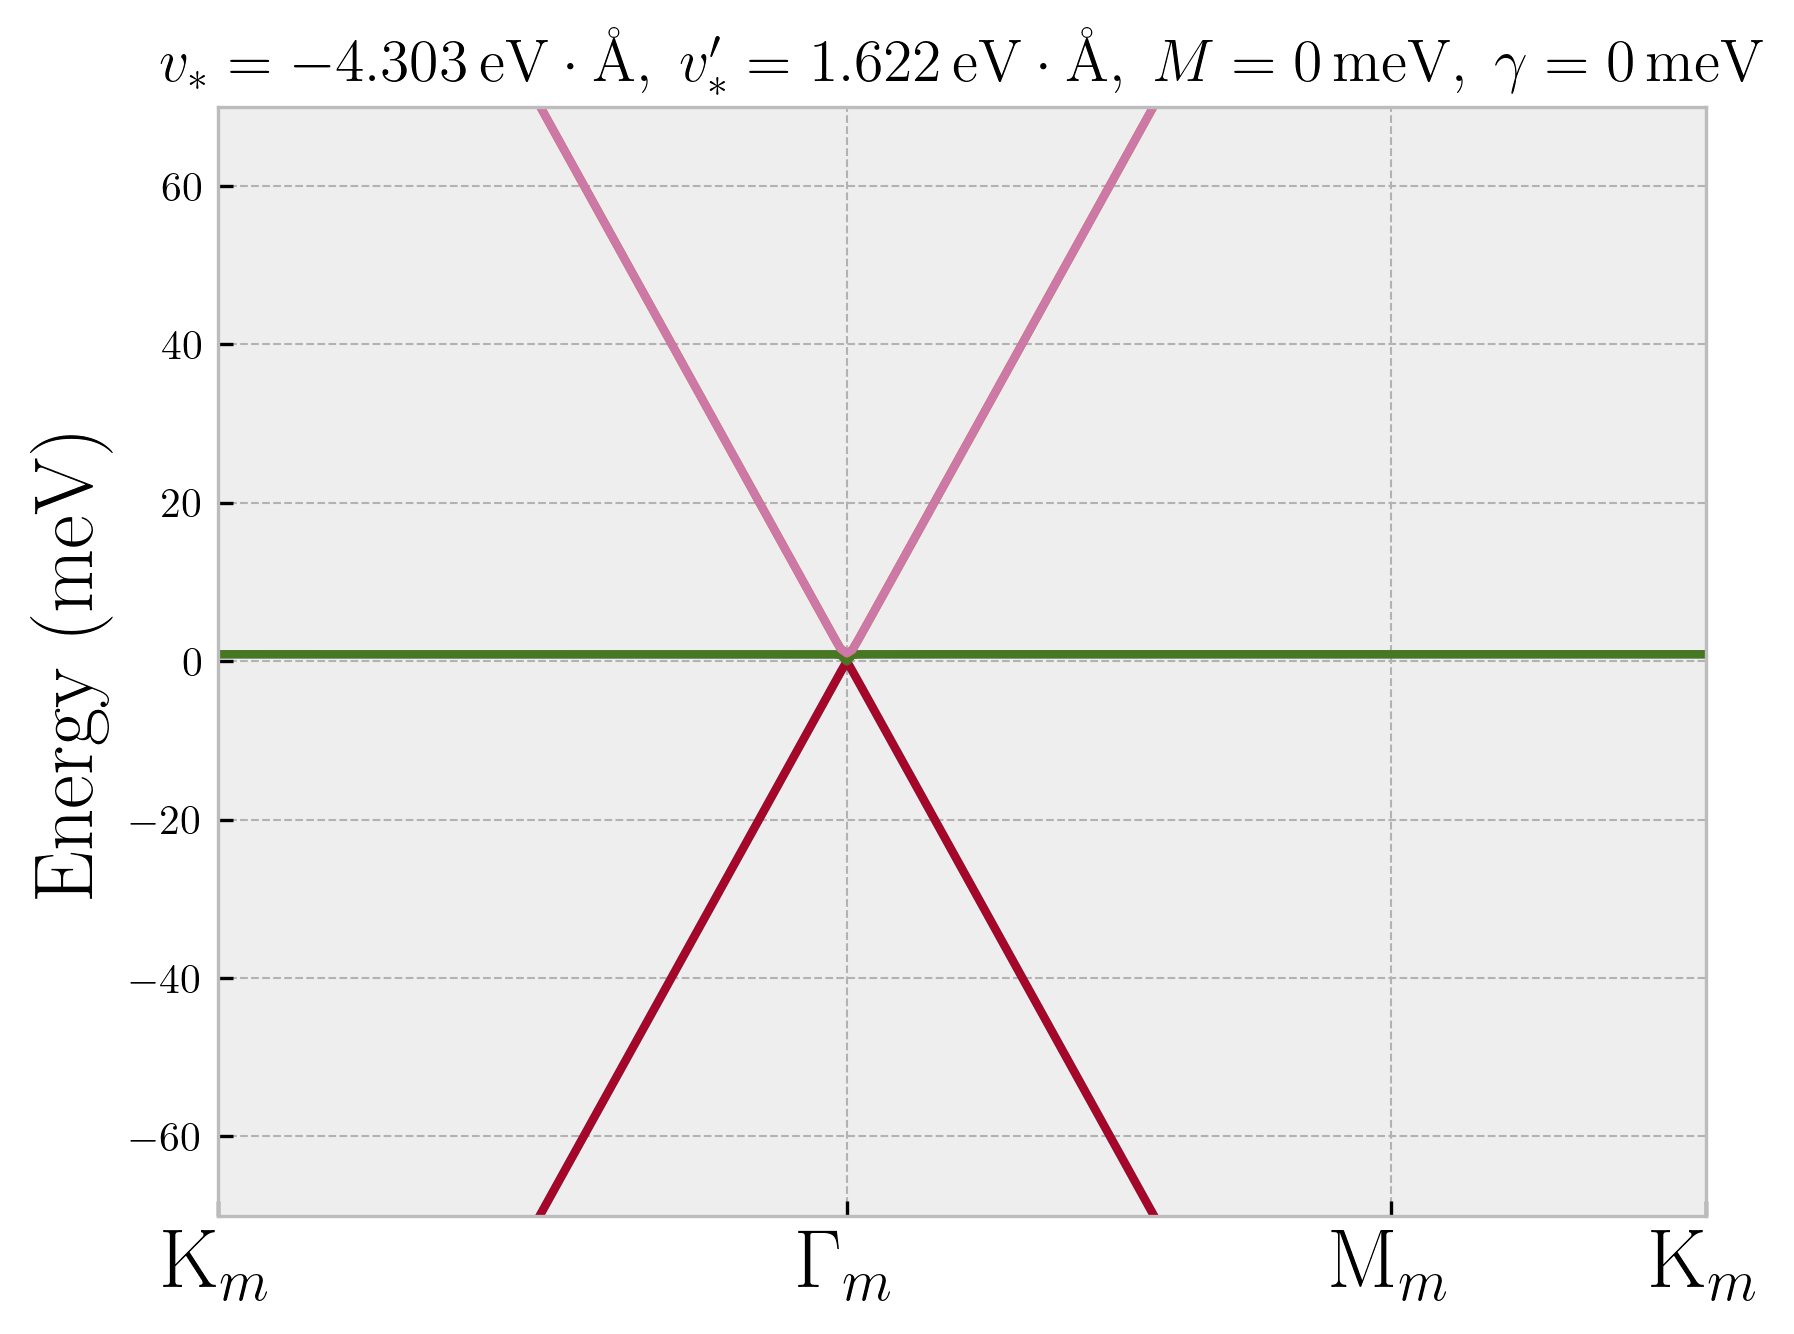
\includegraphics[height=0.35\linewidth]{fig/thf-no_M_no_gamma.png}
%%\caption{}
%\label{fig:thf-correct_params}
%\end{figure}
%\begin{figure}[H]
%\centering
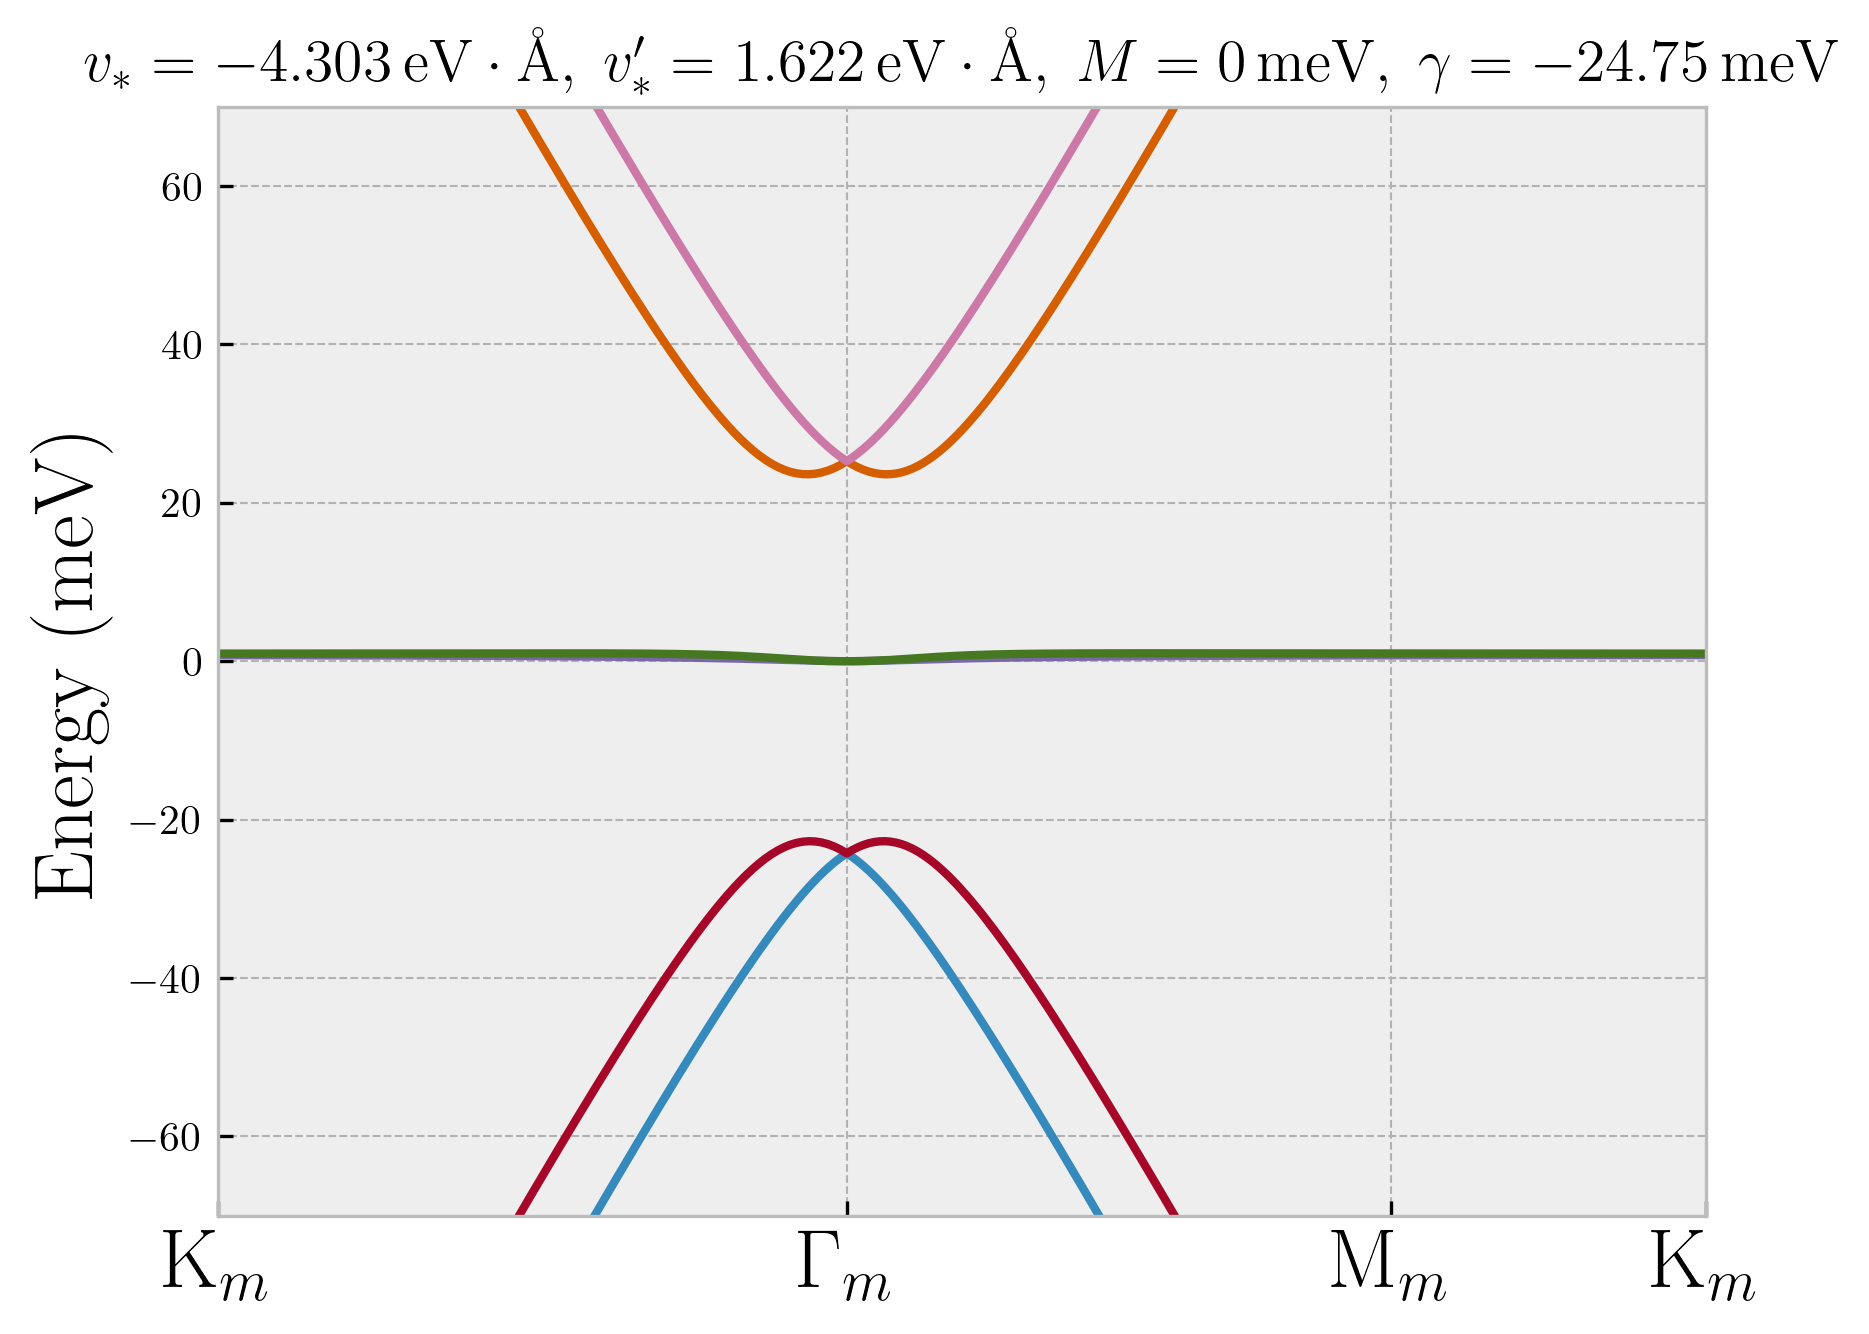
\includegraphics[height=0.35\linewidth]{fig/thf-no_M.png}
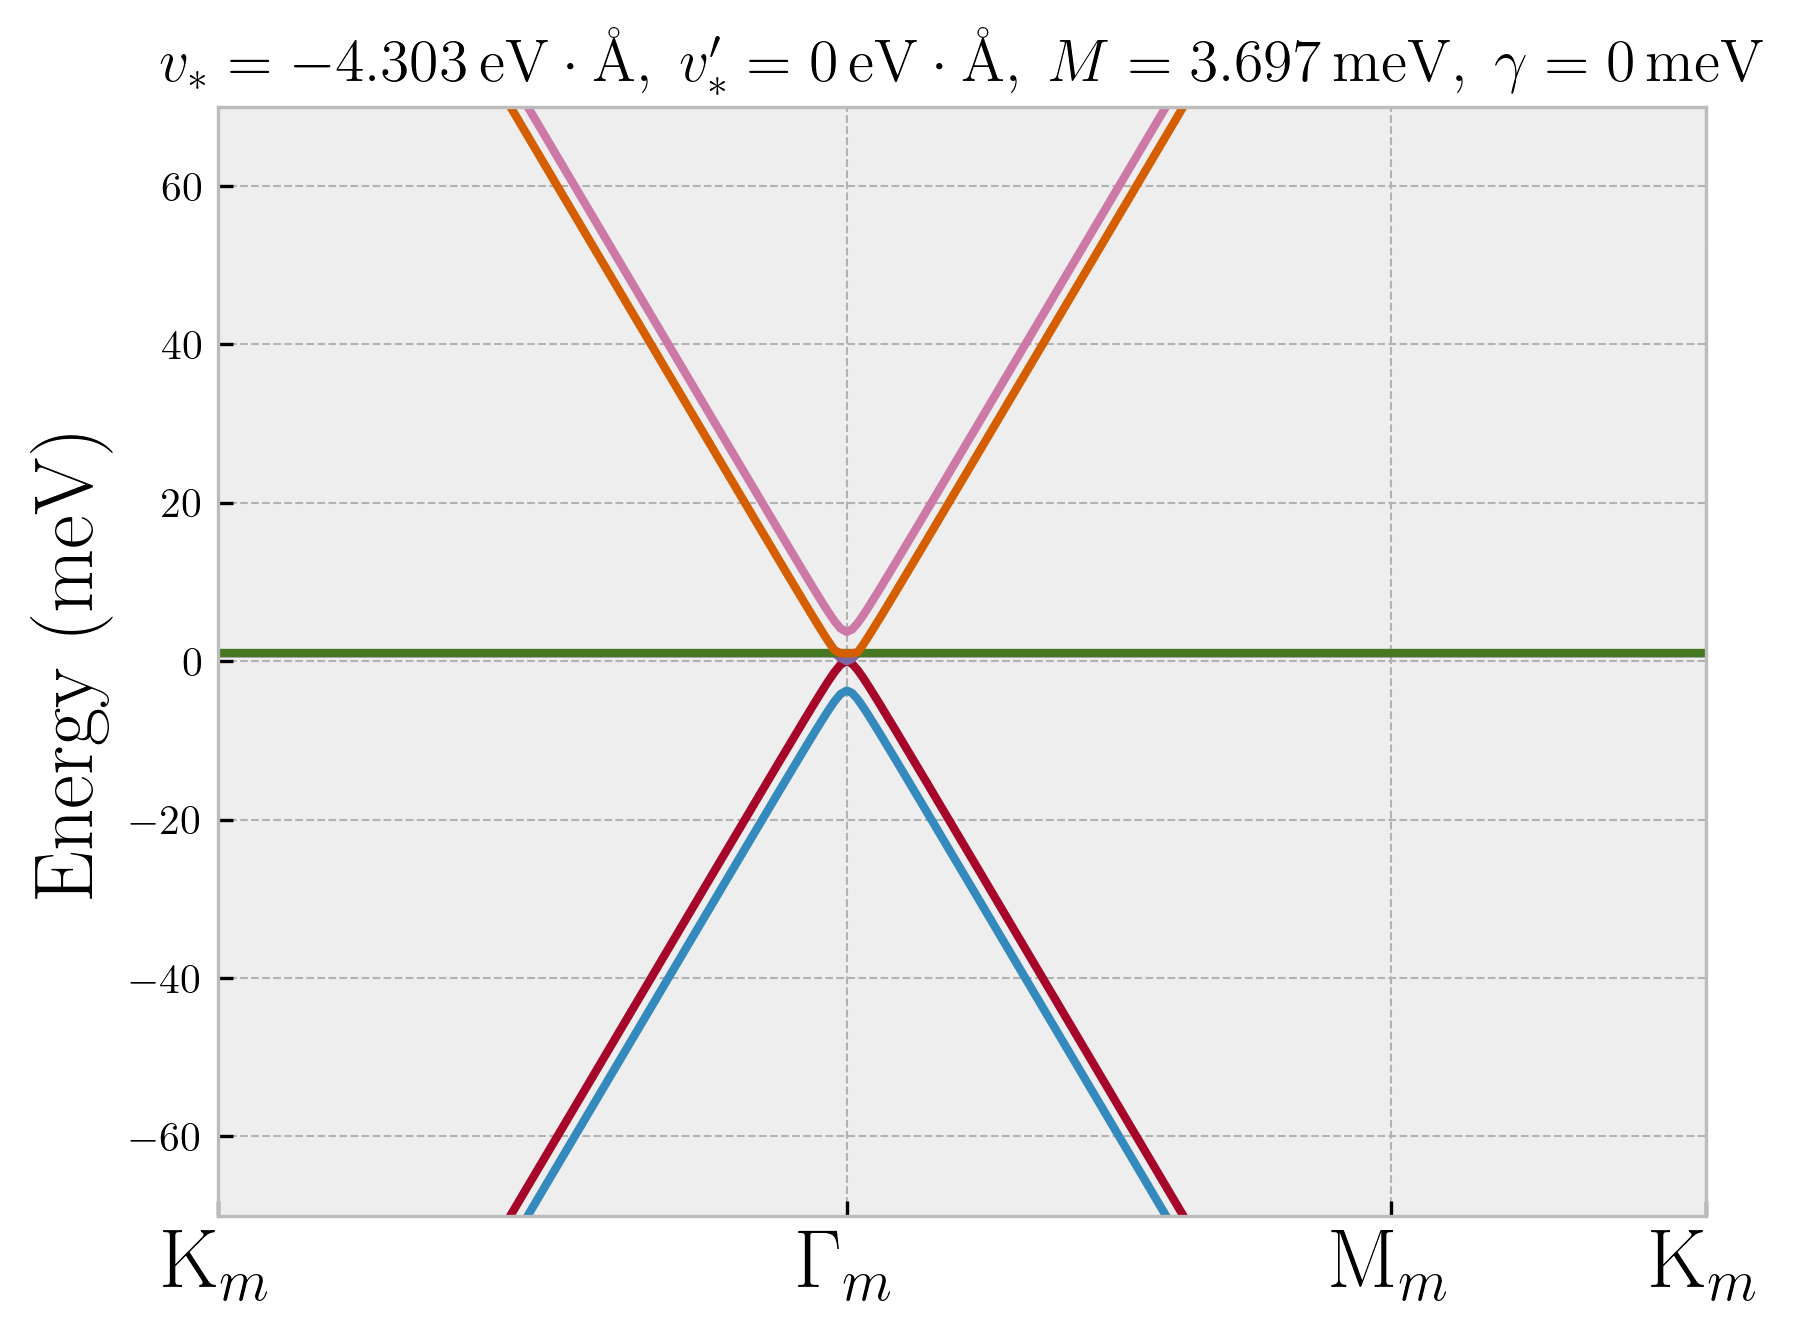
\includegraphics[height=0.35\linewidth]{fig/thf-no_coupling.png}
\caption{Band structures for the 6-band non-interacting Topological Heavy Fermion model.}
\label{fig:thf-exploration}
\end{figure}



%\begin{table}[H]
%\tiny
%\caption{Elementary band representations of the magnetic space group $P6'2'2$.}
%\centering
%\begin{tabular}{|c|c|c|c|c|c|c|c|c|}
%\hline
%Wyckoff & \multicolumn{3}{c|}{$1a$} & \multicolumn{3}{c|}{$2c$} & \multicolumn{2}{c|}{$3f$} \\
%\cline{1-9}
%Site sym. & \multicolumn{3}{c|}{$6'2'2$, $32$} & \multicolumn{3}{c|}{$32$, $32$} & \multicolumn{2}{c|}{$2'2'2$, $2$} \\
%\cline{1-9}
%EBR & $G_{A_1}^{1a}(1)$ & $G_{A_2}^{1a}(1)$ & $G_{E}^{1a}(2)$ & $G_{A_1}^{2c}(2)$ & $G_{A_2}^{2c}(2)$ & $G_{E}^{2c}(4)$   & $G_{A}^{3f}(3)$ & $G_{B}^{3f}(3)$ \\
%\hline
%$\Gamma$ & $\Gamma_1(1)$ & $\Gamma_2(1)$ & $\Gamma_3(1)$ & $2\Gamma_1(1)$ & $2\Gamma_2(1)$ & $2\Gamma_3(2)$ & $\Gamma_1(1)+\Gamma_3(2)$ & $\Gamma_2(1)+\Gamma_3(2)$ \\
%\hline
%$K$ & $K_1(1)$ & $K_1(1)$ & $K_2 K_3(2)$ & $K_2 K_3(2)$ & $K_2 K_3(2)$ & $2K_1(1) + K_2 K_3(2)$ & $K_1(1)+K_2 K_3(2)$ & $K_1(1)+K_2 K_3(2)$ \\
%\hline
%$M$ & $M_1(1)$ & $M_2(1)$ & $M_1(1)+M_2(1)$ & $2M_1(1)$ & $2M_2(1)$ & $2M_1(1)+2M_2(1)$ & $2M_1(1)+M_2(1)$ & $M_1(1)+2M_2(2)$ \\
%\hline
%\end{tabular}
%\label{tab:matbg-irreps}
%\end{table}



%%%%%%%%%%%%%%%%%%%%%%%%%%%%%%%%%%%%%%%%%%%%%%%%%%%%%%%%%%%%%%%%%%%%%%%%%%%%%%%%%%%%%%%%%%%%%%%%%%%
%\section{Monolayer}
%%%%%%%%%%%%%%%%%%%%%%%%%%%%%%%%%%%%%%%%%%%%%%%%%%%%%%%%%%%%%%%%%%%%%%%%%%%%%%%%%%%%%%%%%%%%%%%%%%%
%
%Considering only nearest-neighbors, the hamiltonian of a single unrotated layer of graphene is given by
%$$
%H_{\text{mono}}(\k) = -t
%\begin{pmatrix}
%0 & f(\k) \\
%f^*(\k) & 0
%\end{pmatrix}
%, \quad \ell = 1, 2,
%$$
%where $f = \sum_{i=1}^{3} e^{i \k \vdot \bm{\delta}}$, and $\bm{\delta}$ are the three nearest-neighbor vectors from a site $A$ of the honeycomb lattice.
%
%Expanding in first-order $\k = \K + \q$, where $\K = \frac{4\pi}{3a} (1, 0)$ is the Dirac point of the unrotated layer, we have
%$$
%H_{\text{mono}}(\K + \q) \approx v_F \, \q \vdot \bm{\sigma}.
%$$
%
%%%%%%%%%%%%%%%%%%%%%%%%%%%%%%%%%%%%%%%%%%%%%%%%%%%%%%%%%%%%%%%%%%%%%%%%%%%%%%%%%%%%%%%%%%%%%%%%%%%
%\section{BM model review}
%%%%%%%%%%%%%%%%%%%%%%%%%%%%%%%%%%%%%%%%%%%%%%%%%%%%%%%%%%%%%%%%%%%%%%%%%%%%%%%%%%%%%%%%%%%%%%%%%%%
%
%The hamiltonian of the BM model is given by
%$$
%H = H_1 + H_2 + V + V^\dagger,
%$$
%where $H_1$ and $H_2$ correspond to the layers 1 and 2, and $V$ is the hybridization between them.
%
%\n
%
%For this discussion, we use the reference frame where layer 1 is unrotated and layer 2 is rotated counter-clockwise by an angle $\theta$. Therefore, we have
%$$
%H_1(\k) = H_{\text{mono}}(\k), \quad H_2(\k) = H_1(R_\theta^{-1}\k),
%$$
%$$
%R_\theta =
%\begin{pmatrix}
%\cos\theta & -\sin\theta \\
%\sin\theta & \cos\theta
%\end{pmatrix}.
%$$
%
%Also, the Dirac points of each layer are
%$$
%\K_1 = \K = \frac{4\pi}{3a} (1, 0), \quad \K_2 = R_\theta \K_1 = R_\theta \K,
%$$
%$$
%$$
%
%Therefore, expanding around the Dirac points $\K_1$ and $\K_2$, respectively:
%$$
%H_1(\K_1 + \q) \approx v_F \, \q \vdot \bm{\sigma}.
%$$
%$$
%\boxed{ H_2(\K_2 + \q) = H_2(R_\theta \K_1 + \q) = H_1(\K_1 + R_\theta^{-1}\q) \approx v_F \, (R_\theta^{-1}\q) \vdot \bm{\sigma} \approx v_F \, (1 - i \theta \sigma_y ) \, \q \vdot \bm{\sigma}. }
%$$
%
%If we \textbf{neglect the $\theta$-dependence on $H_2$}, our BM model will be \textbf{particle-hole symmetric}, as defined by Bernevig.
%
%\n
%
%Of course, the more difficult part is due to the hybridization term $V$. It is written on the Bloch basis $\ket{\ell, \alpha, \p}$, where $\ell = 1, 2$ is the layer index, $\alpha = A, B$ is the sublattice index, and $\p$ is the momentum.
%We have
%$$
%V_{\alpha\beta}(\p, \p') = \bra{1, \alpha, \p} H \ket{2, \beta, \p'}.
%$$
%
%When we expand both $\p = \K_1 + \q$ and $\p' = \K_2 + \q'$, \textbf{after the BM considerations}, we get
%$$
%V_{\alpha\beta}(\K + \q, R_\theta \K + \q') \approx
%w \sum_{j=1}^{3} \delta_{\q, \q' + \q_j} T_{\alpha\beta}^j,
%$$
%where $\q_1, \q_2, \q_3$ are the moiré momentum vectors, with absolute value $k_D = 2 \sin(\theta/2) \abs{\K}$. The matrices $T^j_{\alpha\beta}$ are
%$$
%T_1 = \sigma_0 + \sigma_x
%$$
%$$
%T_2 = \sigma_0 + \cos(\frac{2\pi}{3}) \sigma_x + \sin(\frac{2\pi}{3}) \sigma_y
%$$
%$$
%T_3 = \sigma_0 + \cos(\frac{2\pi}{3}) \sigma_x - \sin(\frac{2\pi}{3}) \sigma_y
%$$
%\begin{figure}[H]
%\centering
%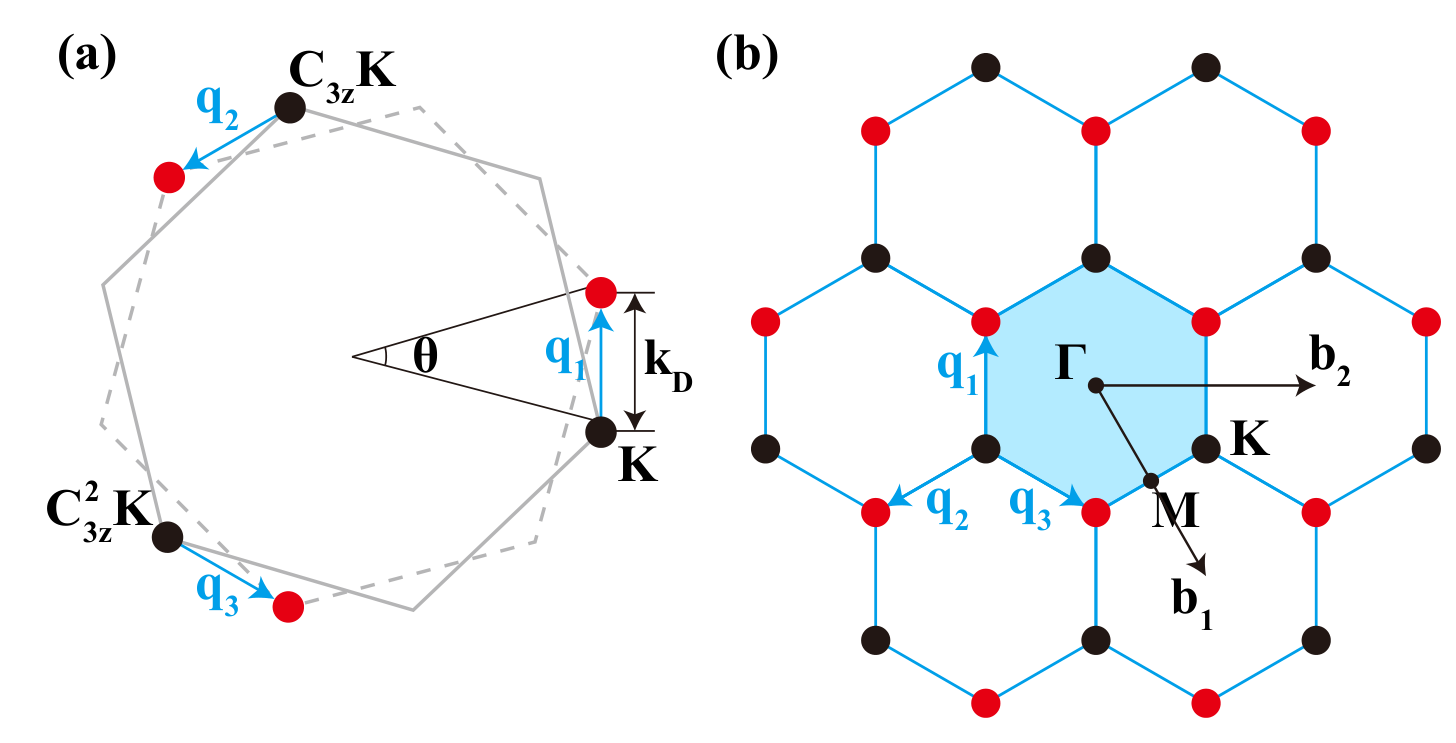
\includegraphics[width=0.8\linewidth]{fig/moire-vectors.png}
%\end{figure}
%
%\n
%
%This \textbf{BM model} is called \textbf{MBM-1V (Moiré Band Model - One Valley)} by Bernevig. If we decompose $\q = \k - \Q$, $\q'=\k-\Q'$, where $\Q$ and $\Q'$ belong to the hexagonal lattice formed by adding $\q_{1,2,3}$ iteratively, we can rewrite the hamiltonian as
%$$
%\boxed{
%H_{\Q, \Q'}^{(\text{MBM-1V})}(\k) =
%\delta_{\Q,\Q'} v_F (\k-\Q) \vdot \bm{\sigma}
%+ w \sum_{j=1}^{3} (\delta_{\Q'-\Q, \q_j} + \delta_{\Q-\Q', \q_j}) T^j.
%}
%$$
%
%\begin{itemize}
%\item This model is \textbf{topological} and is what we have been discussing the whole time.
%\item The tables of Bernevig apply to this model, where we consider the Wyckoff position 1a within the THF approach to solve the topological obstruction.
%\item Its magnetic space group is $P6'2'2$. Generators: $C_{6z} T$, $C_{2y} T$, $C_{2x}$.
%\end{itemize}
%
%\begin{table}[H]
%\scriptsize
%\caption{Elementary band representations of the magnetic space group $P6'2'2$.}
%\centering
%\begin{tabular}{|c|c|c|c|c|c|c|c|c|}
%\hline
%Wyckoff & \multicolumn{3}{c|}{$1a$} & \multicolumn{3}{c|}{$2c$} & \multicolumn{2}{c|}{$3f$} \\
%\cline{1-9}
%Site sym. & \multicolumn{3}{c|}{$6'2'2$, $32$} & \multicolumn{3}{c|}{$32$, $32$} & \multicolumn{2}{c|}{$2'2'2$, $2$} \\
%\cline{1-9}
%EBR & $G_{A_1}^{1a}(1)$ & $G_{A_2}^{1a}(1)$ & $G_{E}^{1a}(2)$ & $G_{A_1}^{2c}(2)$ & $G_{A_2}^{2c}(2)$ & $G_{E}^{2c}(4)$   & $G_{A}^{3f}(3)$ & $G_{B}^{3f}(3)$ \\
%\hline
%$\Gamma$ & $\Gamma_1(1)$ & $\Gamma_2(1)$ & $\Gamma_3(1)$ & $2\Gamma_1(1)$ & $2\Gamma_2(1)$ & $2\Gamma_3(2)$ & $\Gamma_1(1)+\Gamma_3(2)$ & $\Gamma_2(1)+\Gamma_3(2)$ \\
%\hline
%$K$ & $K_1(1)$ & $K_1(1)$ & $K_2 K_3(2)$ & $K_2 K_3(2)$ & $K_2 K_3(2)$ & $2K_1(1) + K_2 K_3(2)$ & $K_1(1)+K_2 K_3(2)$ & $K_1(1)+K_2 K_3(2)$ \\
%\hline
%$M$ & $M_1(1)$ & $M_2(1)$ & $M_1(1)+M_2(1)$ & $2M_1(1)$ & $2M_2(1)$ & $2M_1(1)+2M_2(1)$ & $2M_1(1)+M_2(1)$ & $M_1(1)+2M_2(2)$ \\
%\hline
%\end{tabular}
%\label{tab:ebr-P6'2'2}
%\end{table}
%
%\begin{table}[H]
%\caption{Character table of irreps at high symmetry momenta in magnetic space group $P6'2'2$.}
%\centering
%\begin{tabular} { c c c c | c c c | c c c }
%\cline{1-10}
%$\P$ & $\P \Gamma_1$ & $\P \Gamma_2$ & $\P \Gamma_3$ & $\P$ & $\P M_1$ & $\P M_2$ & $\P$ & $\P K_1$ & $\P K_2K_3$ \\
%\cline{1-10}
%$E$ & $\P1$ & $\P1$ & $\P2$ & $\P E$ & $\P1$ & $\P1$ & $\P E$ & $\P1$ & $\P2$ \\
%$2 C_3$ & $\P1$ & $\P1$ & $ -1$ & $\P C_2'$ & $\P1$ & $ -1$ & $\P C_3$ & $\P1$ & $ -1$ \\
%$3 C_2'$ & $\P1$ & $ -1$ & $\P0$ & $\P$ & $\P$ & $\P$ & $\P C_3^{-1}$ & $\P1$ & $-1$ \\
%\cline{1-10}
%\end{tabular}
%\label{tab:char-P6'2'2}
%\end{table}



%%%%%%%%%%%%%%%%%%%%%%%%%%%%%%%%%%%%%%%%%%%%%%%%%%%%%%%%%%%%%%%%%%%%%%%%%%%%%%%%%%%%%%%%%%%%%%%%%%%
%\section{There exists another model}
%%%%%%%%%%%%%%%%%%%%%%%%%%%%%%%%%%%%%%%%%%%%%%%%%%%%%%%%%%%%%%%%%%%%%%%%%%%%%%%%%%%%%%%%%%%%%%%%%%%
%
%According to Bernevig: ``The MBM-1V is half of the TBG system, with similar physics taking place in the electron states around $\K'$''. A model with the two valleys can be written as
%$$
%\boxed{
%H_{\Q, \Q'}^{(\text{MBM-2V})}(\k) =
%\delta_{\Q,\Q'} v_F (\k-\Q) \vdot \bm{\sigma} \otimes \tau_z
%+ w \sum_{j=1}^{3} (\delta_{\Q'-\Q, \q_j} + \delta_{\Q-\Q', \q_j}) T^j \otimes \tau_0.
%}
%$$
%
%Here $\tau_z$ and $\tau_0$ are the Pauli and identity matrix representing the valley degree of freedom.
%
%\begin{itemize}
%\item This model is \textbf{apparently different} from the latter, and \textbf{is not topological}. You can decompose it in EBR's as $G_{A_1}^{2c} + G_{A_2}^{2c}$.
%\item The tables of Rennella apply to this model. There the authors (Vafek, Rennella, Angeli, Koshino, etc) consider Wyckoff position 2c, because these positions really correspond to symmetry-adapted exponentially localized Wannier functions.
%\item The magnetic space group is $P6221'$. Generators: $C_{6z}$, $C_{2y}$, $C_{2x}$, $T$.
%\end{itemize}
%
%\begin{table}[H]
%\caption{Elementary band representations generated from Wyckoff position $2c$ of the space group $P622$.}
%\centering
%\begin{tabular}{|c|c|c|c|}
%\hline
%Wyckoff & \multicolumn{3}{c|}{$2c$} \\
%\cline{1-4}
%Site sym. & \multicolumn{3}{c|}{$32$} \\
%\cline{1-4}
%EBR & $G_{A_1}^{2c}(2)$ & $G_{A_2}^{2c}(2)$ & $G_{E}^{2c}(4)$  \\
%\hline
%$\Gamma$ & $\Gamma_1(1) + \Gamma_4(1)$ & $\Gamma_2(1) + \Gamma_3(1)$ & $\Gamma_5(2) + \Gamma_6(2)$ \\
%\hline
%$K$ & $K_3(2)$ & $K_3(2)$ & $K_1(1) + K_2(1) + K_3(2)$ \\
%\hline
%$M$ & $M_1(1) + M_4(1)$ & $M_2(1) + M_3(1)$ & $M_1(1) + M_2(1) + M_3(1) + M_4(1)$ \\
%\hline
%\end{tabular}
%\label{tab:ebr-P622}
%\end{table}
%
%\begin{table}[H]
%\caption{Character table of irreps at high symmetry momenta in space group $P622$.}
%\scriptsize
%\centering
%\begin{tabular} { c c c c c c c | c c c c c | c c c c }
%\cline{1-16}
%$\P$ & $\P \Gamma_1$ & $\P \Gamma_2$ & $\P \Gamma_3$ & $\P \Gamma_4$ & $\P \Gamma_5$ & $\P \Gamma_6$ & $\P$ & $\P M_1$ & $\P M_2$ & $\P M_3$ & $\P M_4$ & $\P$ & $\P K_1$ & $\P K_2$ & $\P K_3$\\
%\cline{1-16}
%$E$      & $\P1$ & $\P1$ & $\P1$ & $\P1$ & $\P2$ & $\P2$ & $E$     & $\P1$ & $\P1$  & $\P1$ & $\P1$ & $E$      & $\P1$ & $\P1$ & $\P2$ \\
%$2C_6$   & $\P1$ & $\P1$ & $ -1$ & $ -1$ & $ -1$ & $\P1$ & $C_2$   & $\P1$ & $\P1$  & $ -1$ & $ -1$ & $C_3$    & $\P1$ & $\P1$ & $ -1$ \\
%$2C_3$   & $\P1$ & $\P1$ & $\P1$ & $\P1$ & $ -1$ & $ -1$ & $C_2'$  & $\P1$ & $ -1$  & $ -1$ & $\P1$ & $3C_2''$ & $\P1$ & $ -1$ & $\P0$ \\
%$C_2$    & $\P1$ & $\P1$ & $ -1$ & $ -1$ & $\P2$ & $ -2$ & $C_2''$ & $\P1$ & $ -1$  & $\P1$ & $ -1$ &          &       &       &       \\
%$3C_2'$  & $\P1$ & $ -1$ & $ -1$ & $\P1$ & $\P0$ & $\P0$ &         &       &        &       &       &          &       &       &       \\
%$3C_2''$ & $\P1$ & $ -1$ & $\P1$ & $ -1$ & $\P0$ & $\P0$ &         &       &        &       &       &          &       &       &       \\
%\cline{1-16}
%\end{tabular}
%\label{tab:char-P622}
%\end{table}
%
%Compare tables \ref{tab:ebr-P622} and \ref{tab:char-P622} with tables 2.5 and (2.1, 2.3) of Rennella \cite{thesis_rennella}, respectively.

\chapter{Evaluation of the Institutional Support received during the period} \label{chp:apoioInst}
%\chapter{Description and evaluation of the Institutional Support received during the period} \label{chp:apoioInst}

During the period covered by this report, the student used the research overhead to reimburse the remaining cost of the Acer Nitro 5 AN515-58-58W3 laptop. This laptop was originally purchased during the first year of the FAPESP project, but the funds available at that time were insufficient to cover the full amount. The laptop has been extensively used for project-related work and numerical calculations.



\chapter{Participation in scientific events} \label{chp:particEvento}

During the period covered by this report, the student did not participate in any formal scientific events. However, the student attended Luis Gregorio Dias' group meetings and a meeting with collaborators from Eduardo Miranda's group (IFGW-Unicamp), associated with the Thematic Project ``Correlated Quantum Materials'' (\#\texttt{2022/15453-0}).


\chapter{Conclusions and Future Activities} \label{chp:conclusions}

%In Section \ref{sec:tbg}, we presented our research on TBG theory. We derived the Bistritzer-MacDonald model \cite{macdonald2011} in Section \ref{sec:BM-model}. Our intention is to utilize this knowledge to develop our own code for analyzing the electronic properties of the system. The BM model is advantageous as it is independent of whether a configuration of TBG is commensurate or not, and it also incorporates all the emergent symmetries observed in experiments \cite{zou2018}. In order to construct the Wannier orbitals localized on the AB and BA regions of interest, we recognized the necessity of thoroughly reviewing concepts of group theory in Section \ref{sec:grouptheory}. Our studies will enable us to employ group theory to elucidate the Wannier Obstruction \cite{zou2018} and the Topological Heavy Fermion model \cite{topoheavyfermion2022}.
%
%In Section \ref{sec:hubbard}, we established a fully operational DMFT algorithm and extensively explored the phase diagrams for the Metal-Insulator transition. In Figure \ref{fig:UxT-rho0}(a), we successfully replicated a known result from the literature for $\eps_d = U/2$ \cite{georges1996}. Additionally, we conducted a thorough investigation of the asymmetric case, which has received comparatively less attention in the literature. Notably, we analyzed the expansion of the coexistence region as we deviated from the particle-hole symmetric (PHS) case and observed the distinctive ``smile'' pattern in the $U \times \eps_d$ phase diagrams of Figure \ref{fig:T0002-butterfly}. Looking ahead to our DMFT progress, our goal is to enhance and extend the algorithm for the study of TBG. However, before developing a practical implementation, we acknowledge the necessity of comprehensively understanding the intrinsic properties of the system through a rigorous analysis of its symmetries.

%%-----
%% Referências bibliográficas
%%-----
\addcontentsline{toc}{chapter}{\bibname}
%\bibliographystyle{abntex2-num}
\bibliography{bibliografia}
\bibliographystyle{ieeetr}


%%-----
%% Fim do documento
%%-----

\end{document}
